%!TEX root = ../StrinJet.tex

\section{Simulate with PYTHIA 8 sQCD with CR1 and rope}%
\label{sec:CRorRope}

\begin{figure}[t]
        \begin{center}
                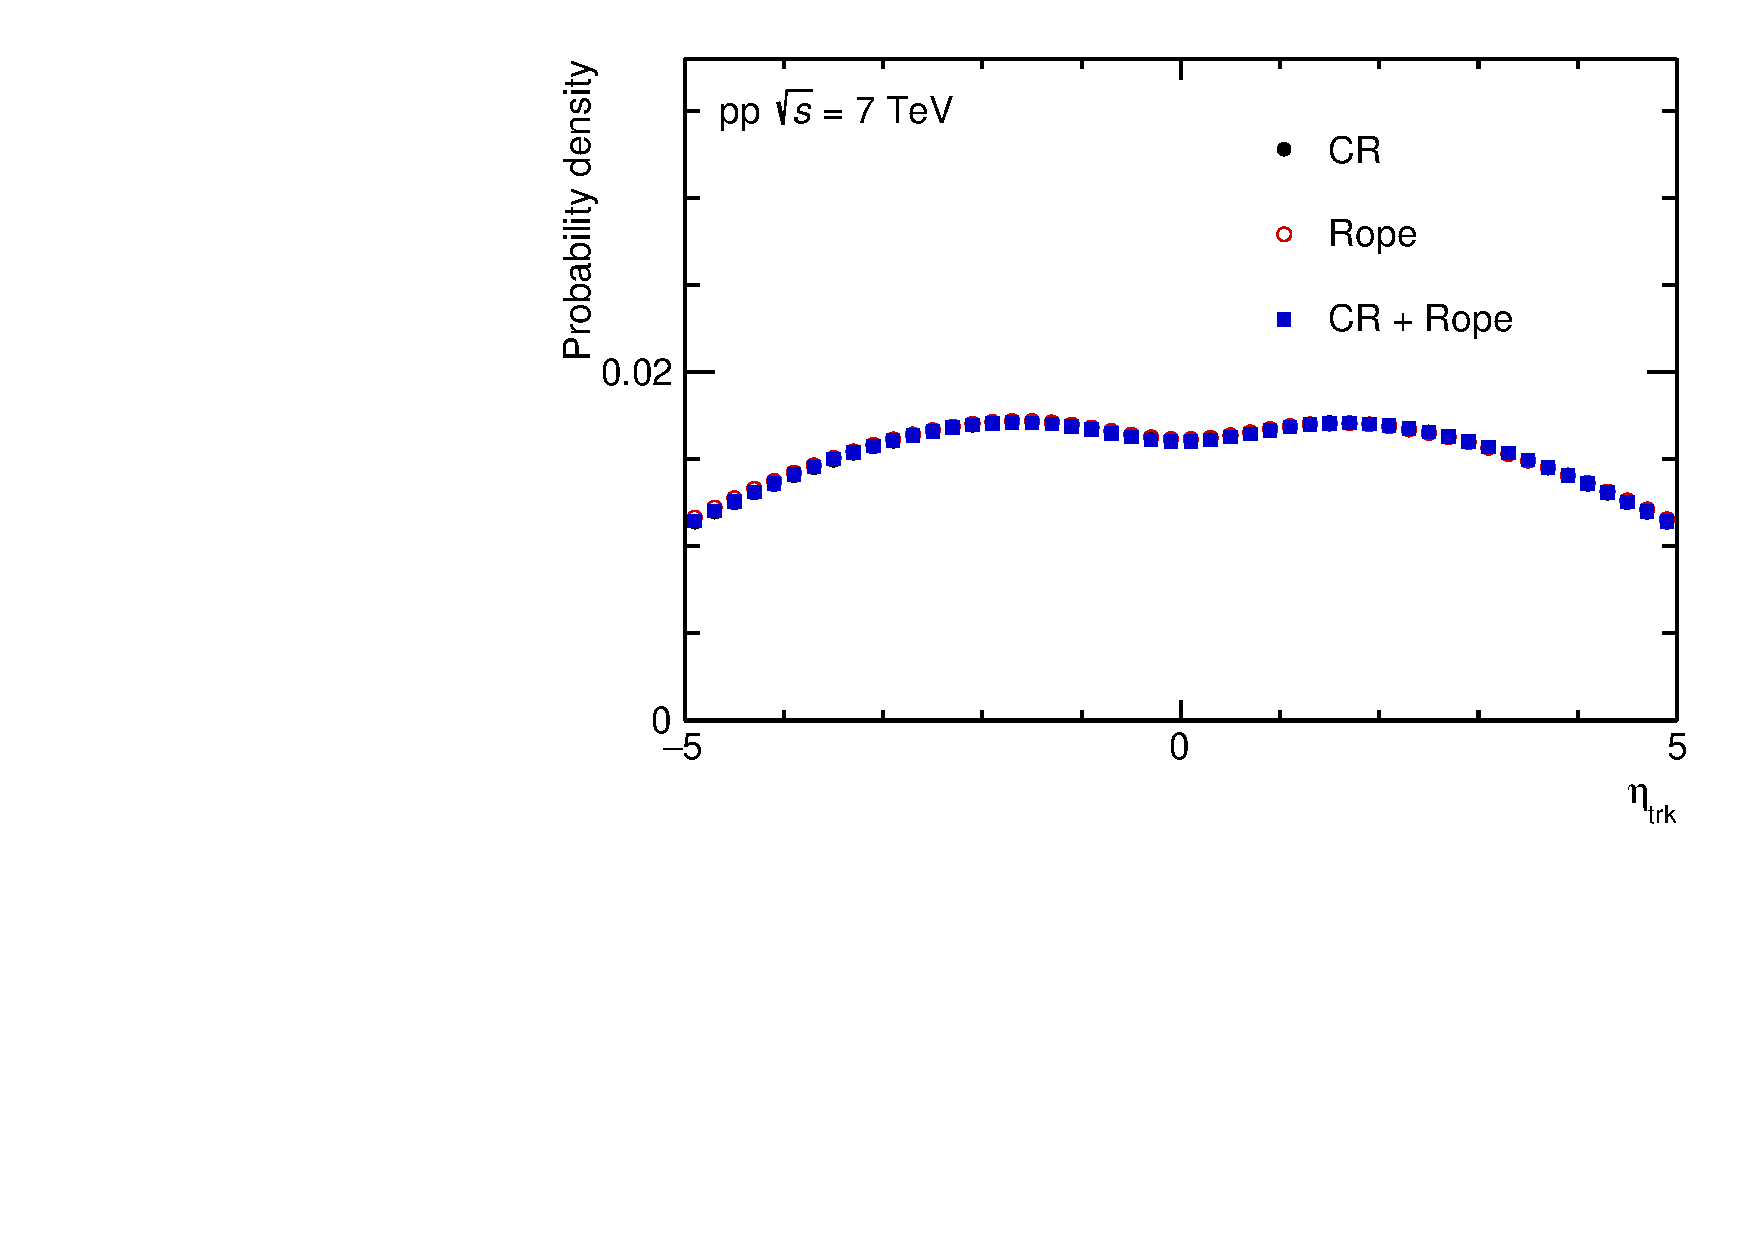
\includegraphics[width=.6\textwidth]{TrkEta}
        \end{center}
        \caption{Track $\eta$ distribution.}
        \label{fig:TrkEta}
\end{figure}

\begin{figure}[t]
	\begin{center}
		%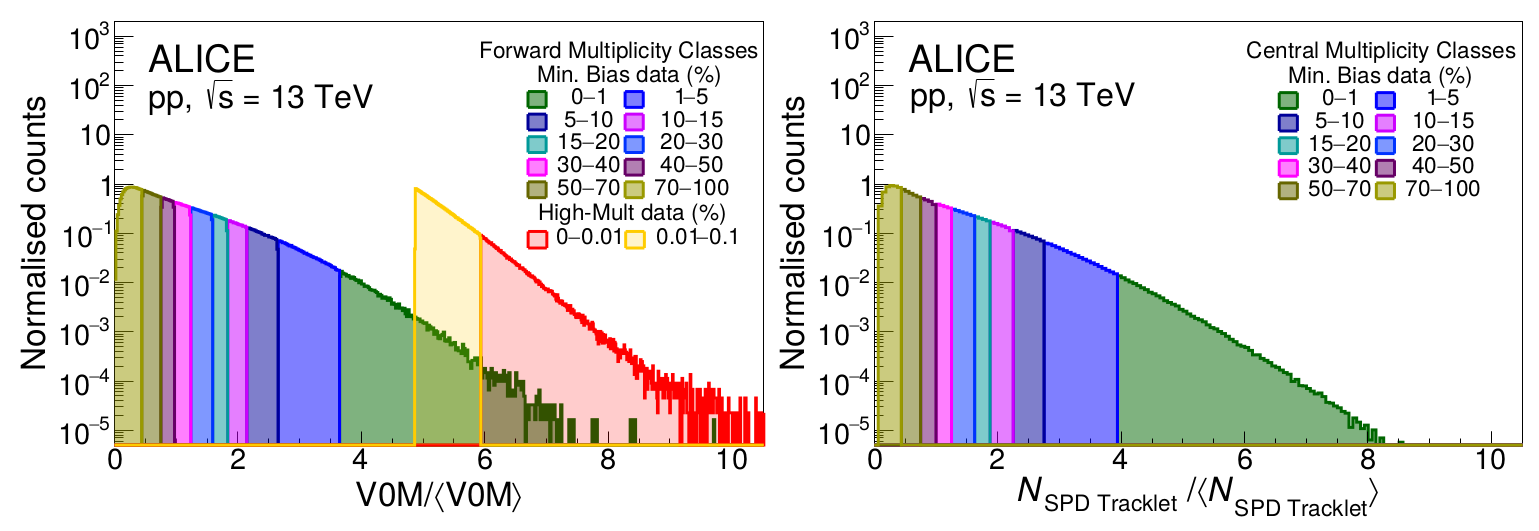
\includegraphics[width=.96\textwidth]{Multiplicity}
		%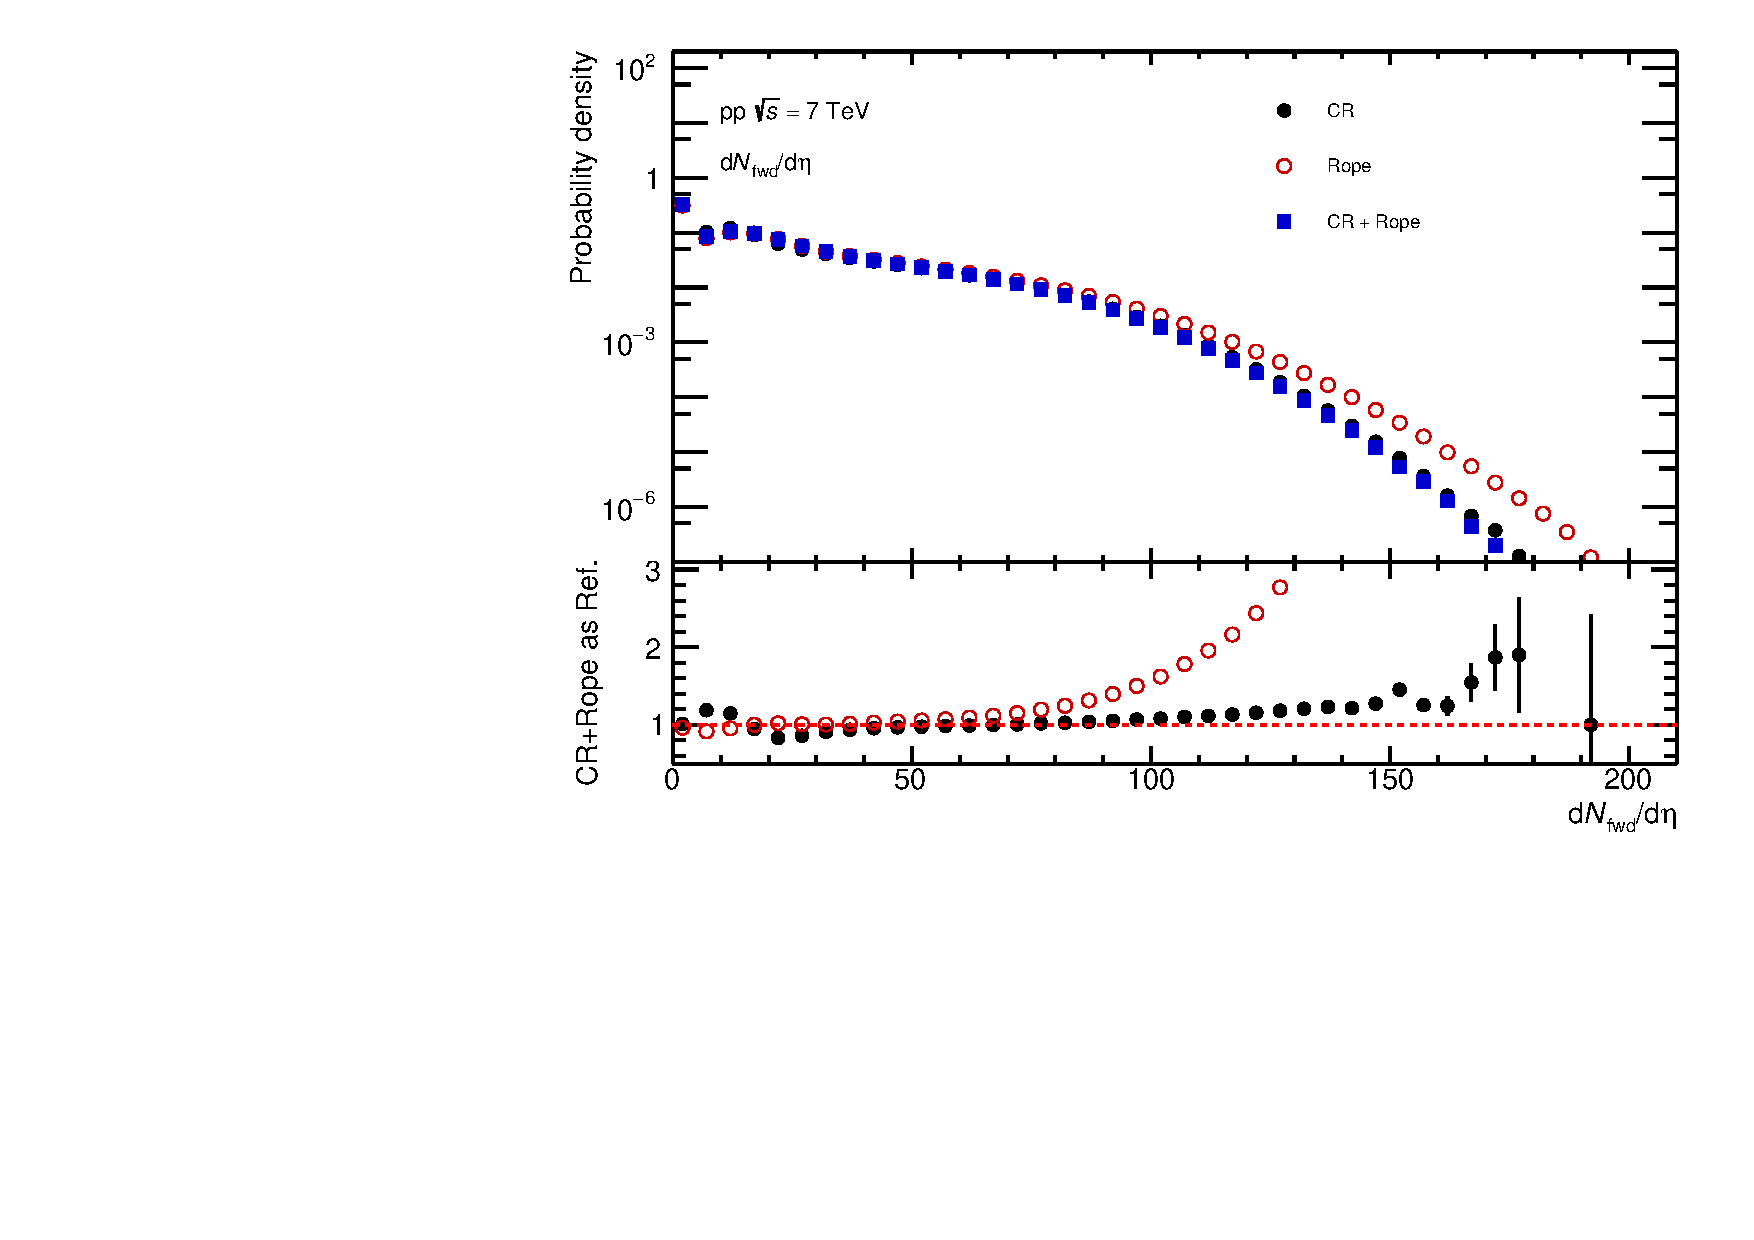
\includegraphics[width=.48\textwidth]{dNfwddEta}
		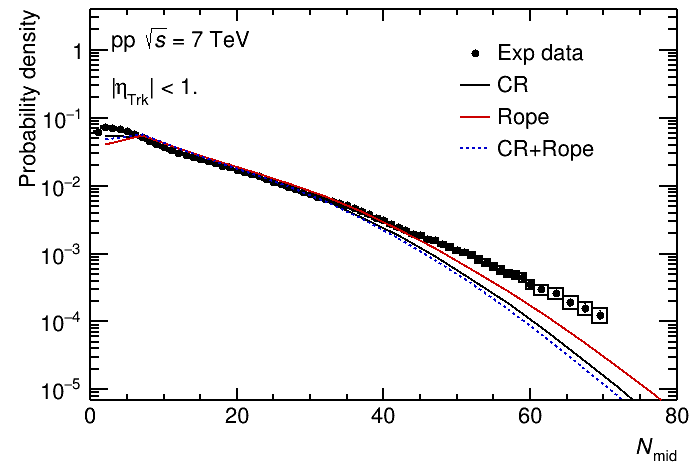
\includegraphics[width=.6\textwidth]{dNmiddEta}
	\end{center}
	\caption{$N_\mathrm{fwd}/\langle N_\mathrm{fwd}\rangle$(left) and $N_\mathrm{mid}/\langle N_\mathrm{mid}\rangle$(right) distribution.(Data got from arXiv:2009.09434)}
	\label{fig:TrkdNdEta}
\end{figure}

%===================================================================
\begin{figure}[ht]
	\begin{center}
		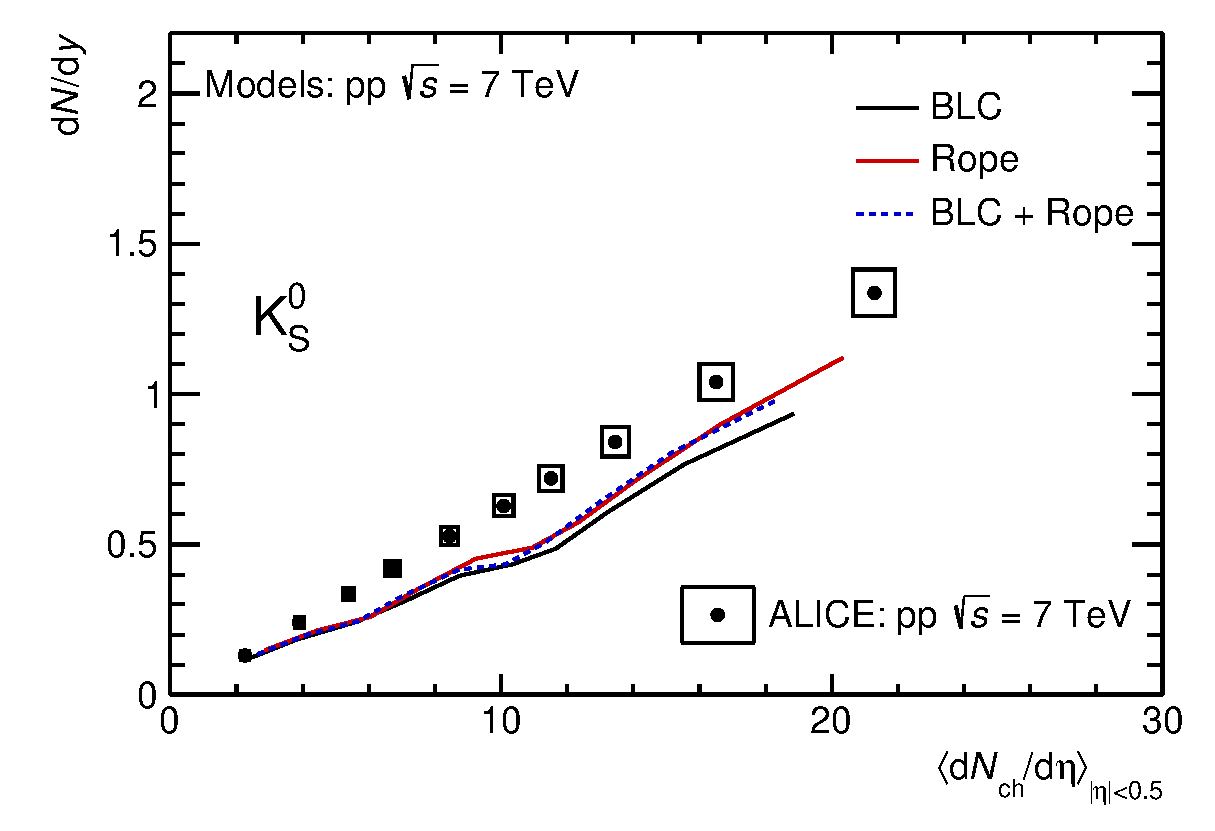
\includegraphics[width=.48\textwidth]{Kshort_InteSpectrum}
		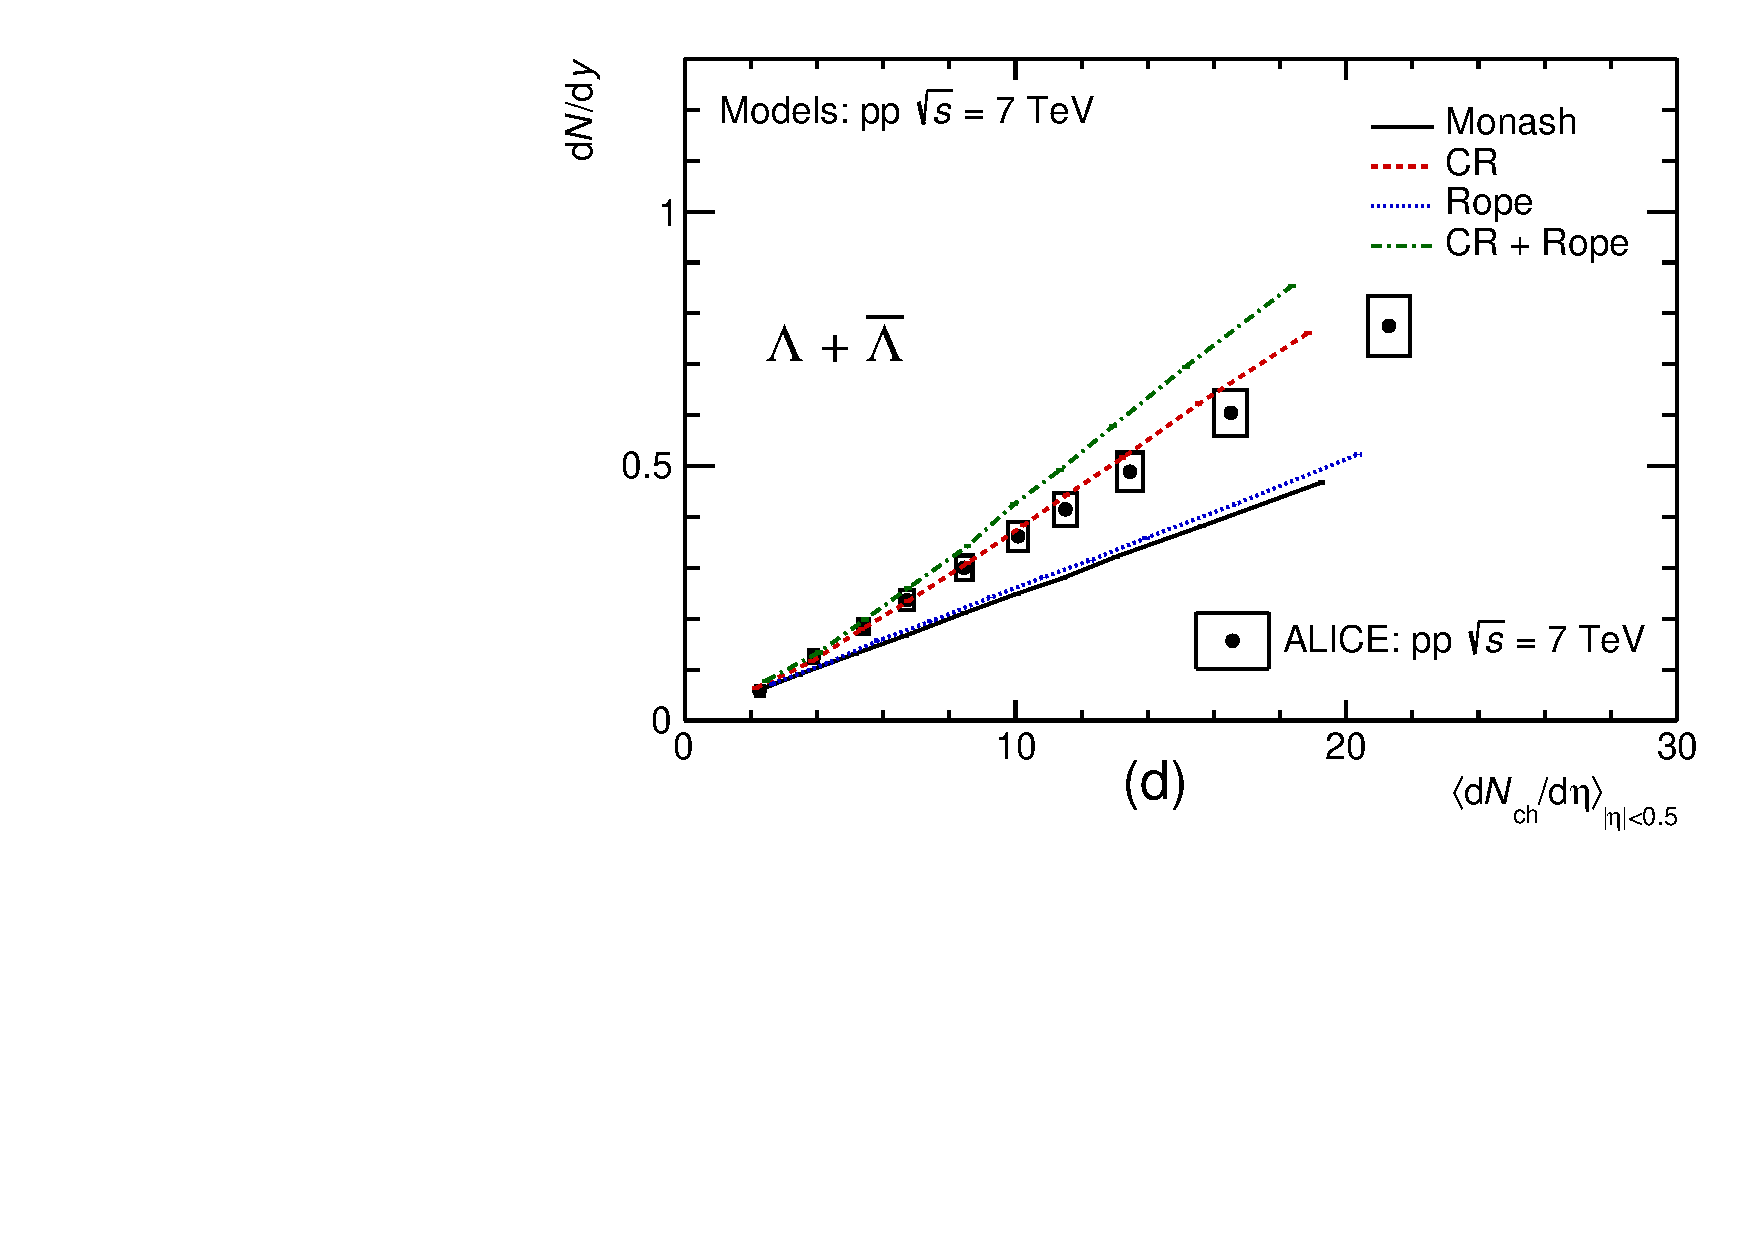
\includegraphics[width=.48\textwidth]{Lambda_InteSpectrum}
		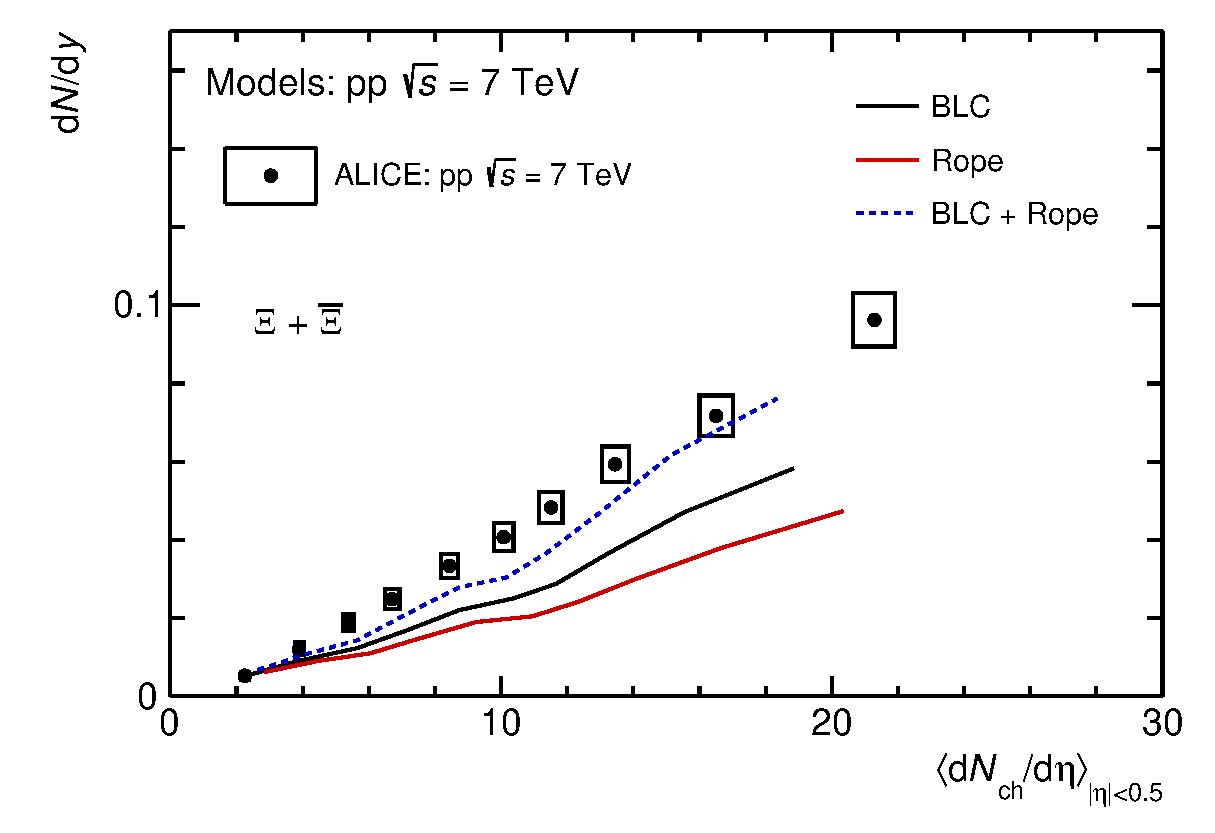
\includegraphics[width=.48\textwidth]{Xi_InteSpectrum}
		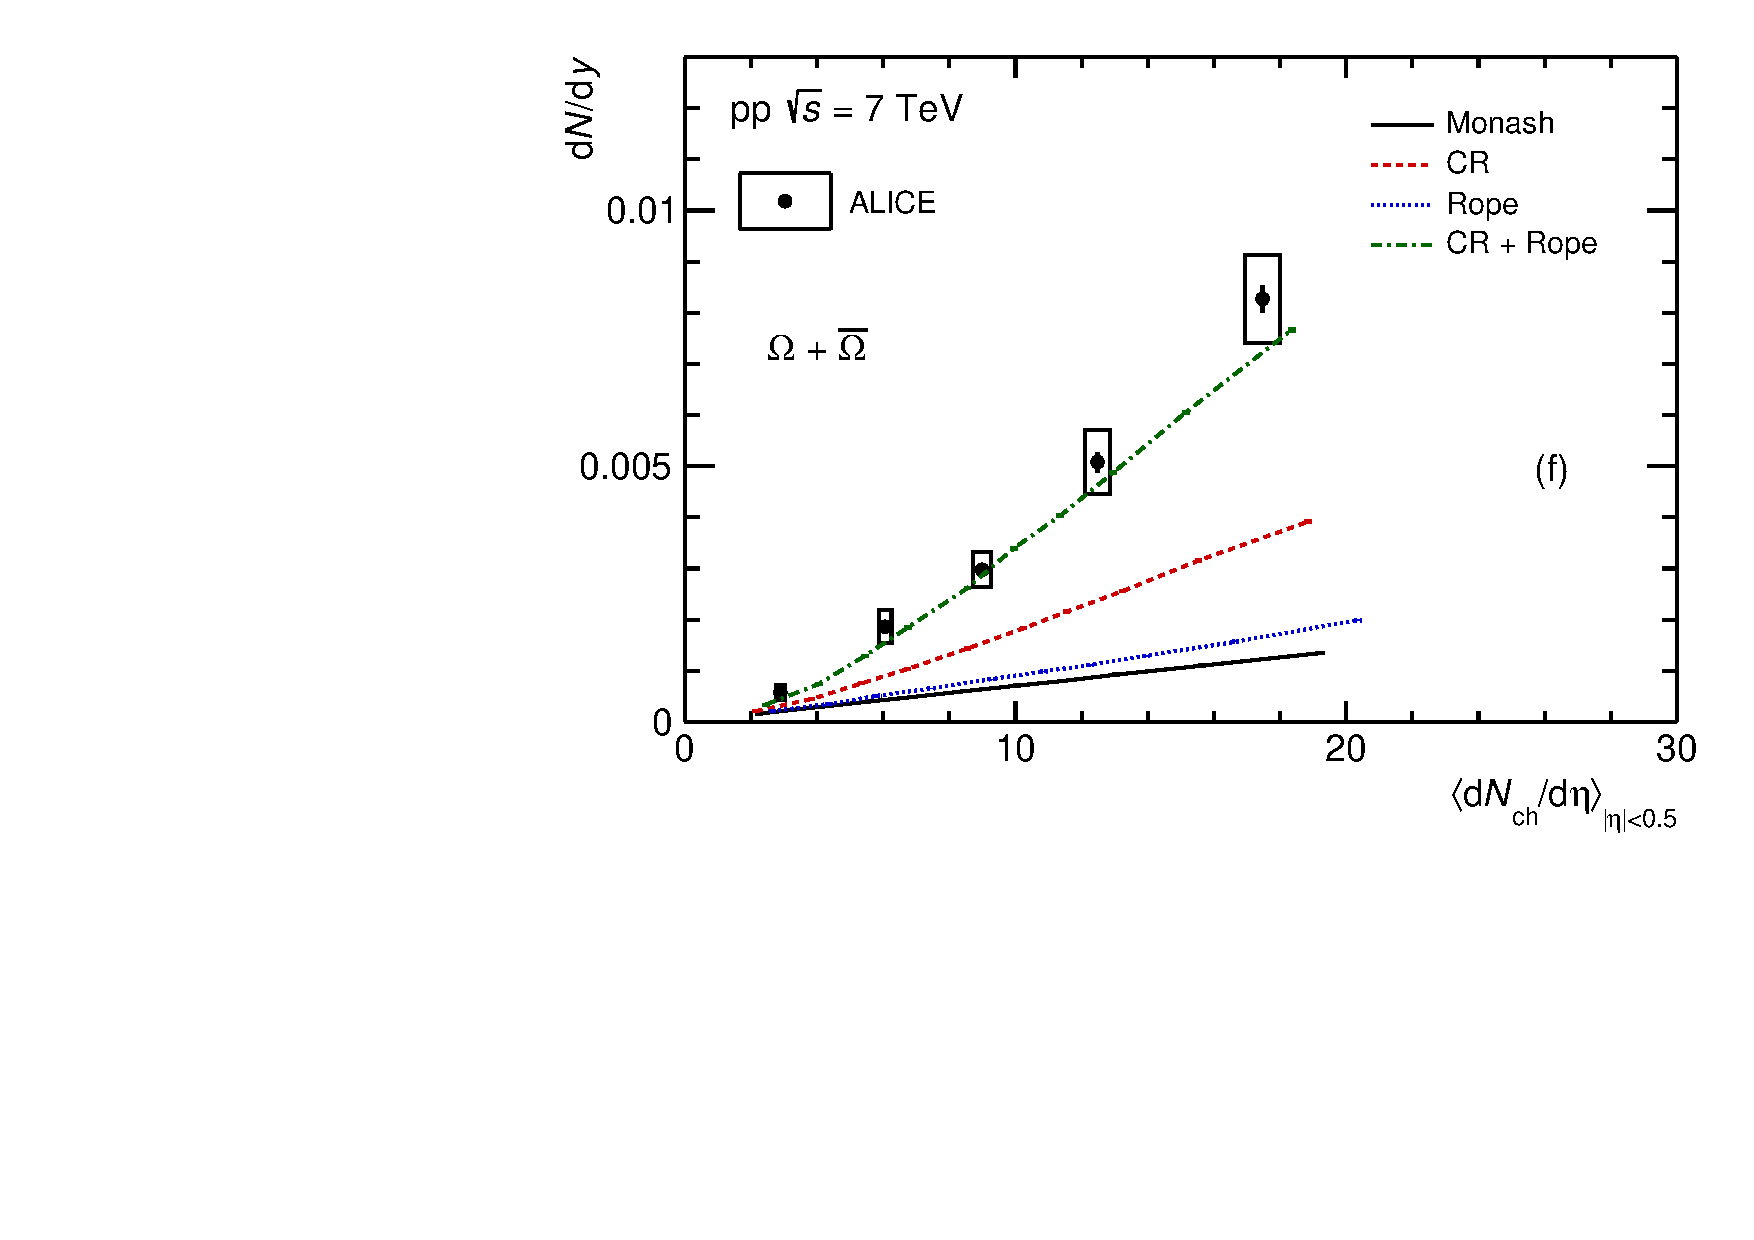
\includegraphics[width=.48\textwidth]{Omega_InteSpectrum}
		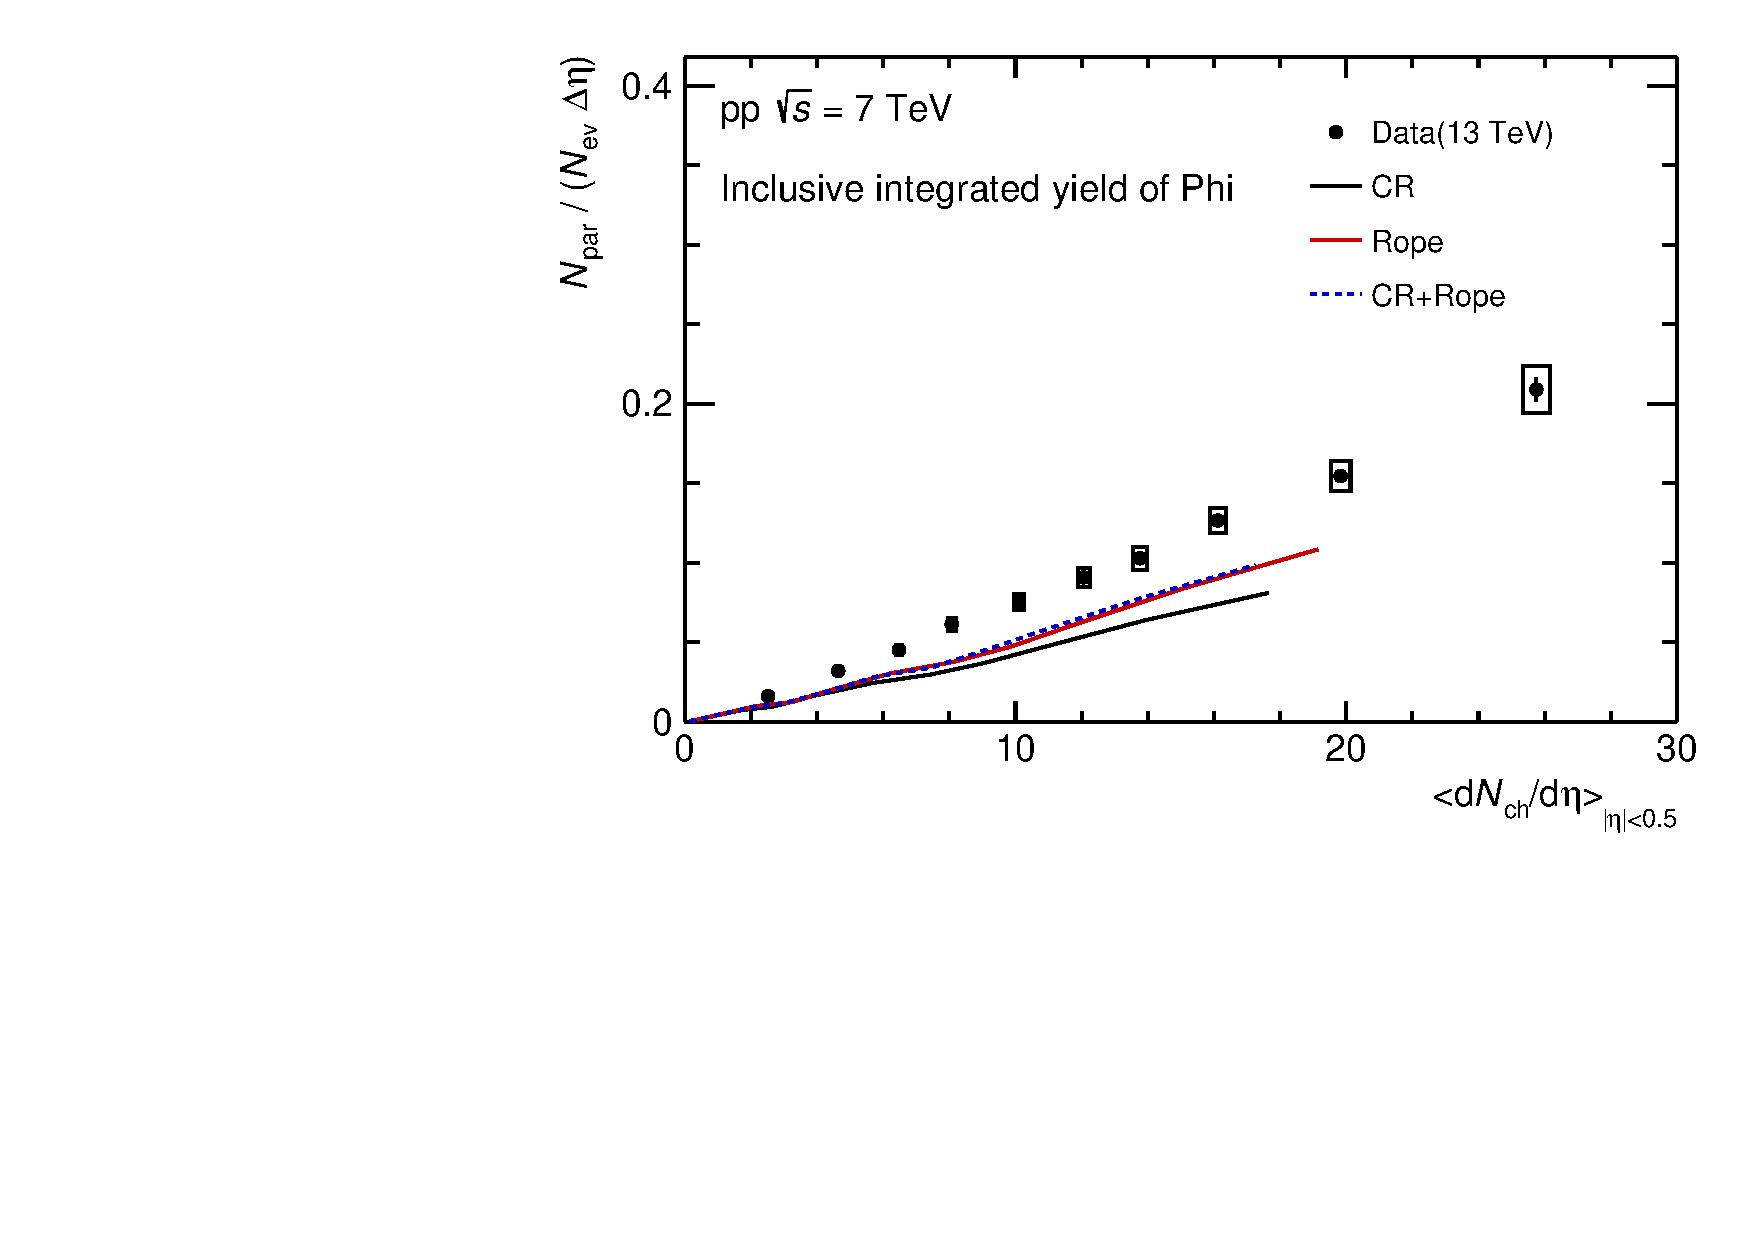
\includegraphics[width=.48\textwidth]{Phi_InteSpectrum}
		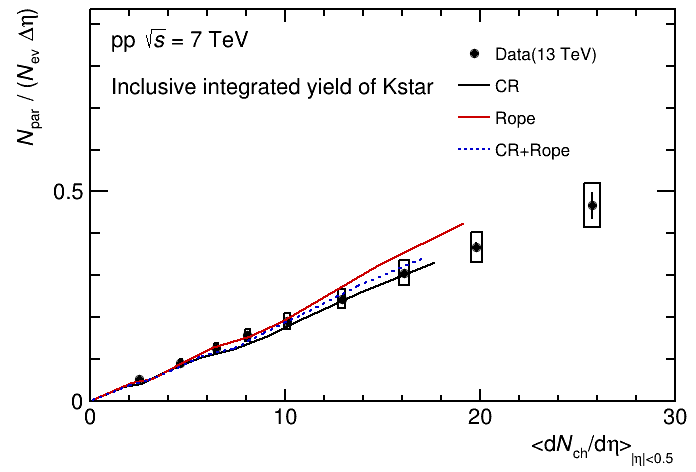
\includegraphics[width=.48\textwidth]{Kstar_InteSpectrum}
		%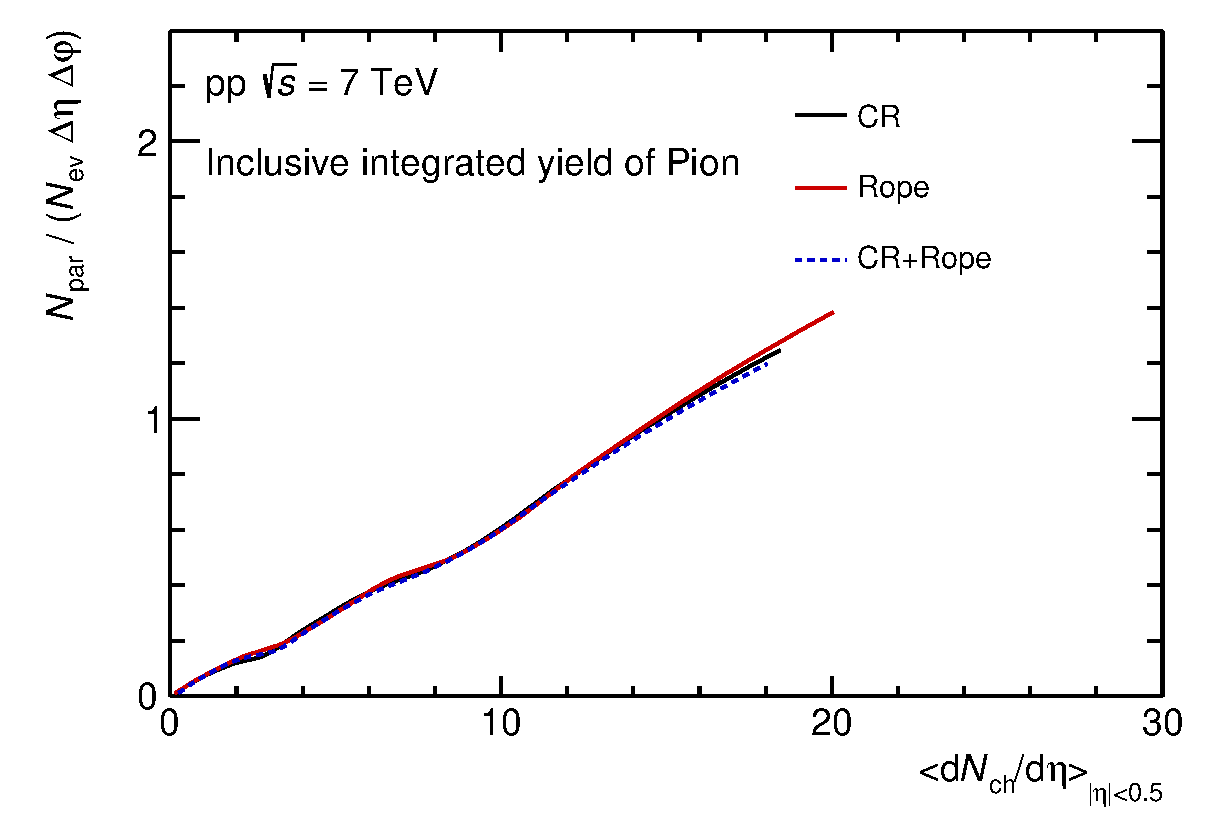
\includegraphics[width=.48\textwidth]{Pion_InteSpectrum}
		%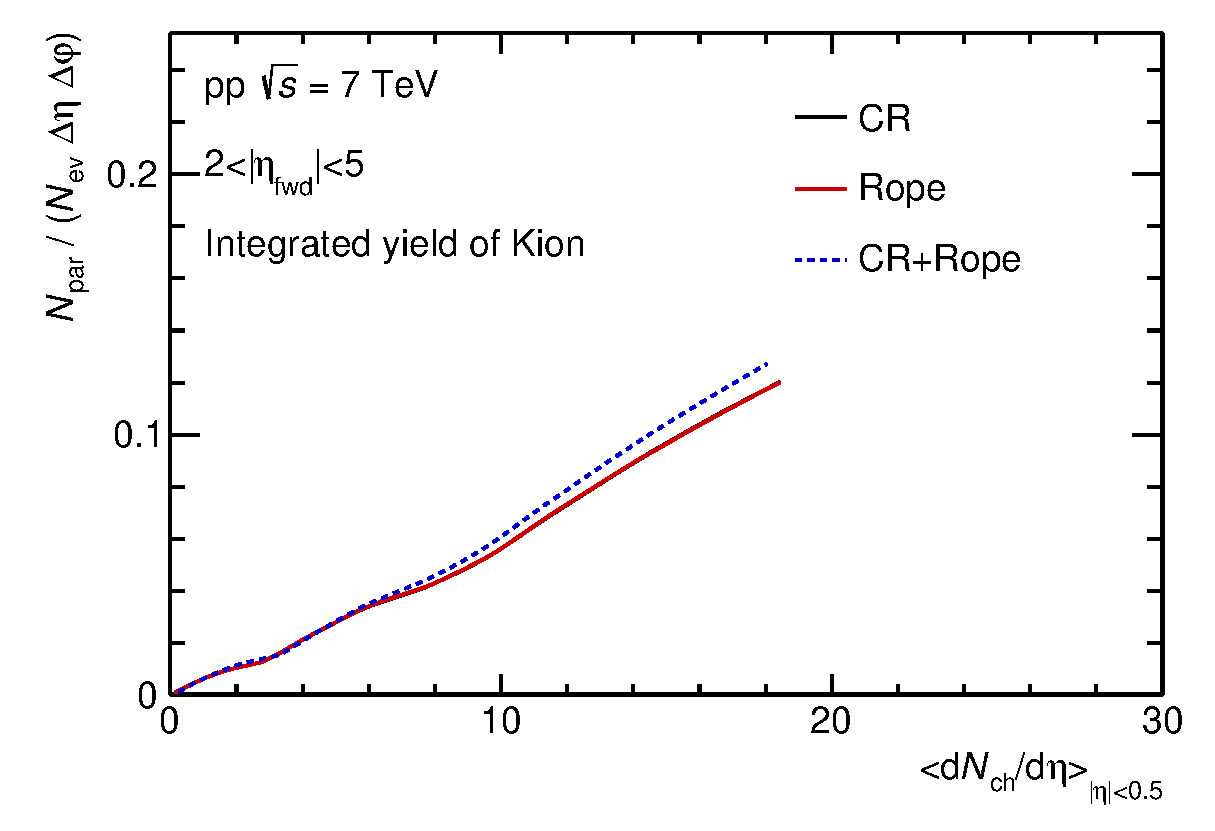
\includegraphics[width=.48\textwidth]{Kion_InteSpectrum}
		%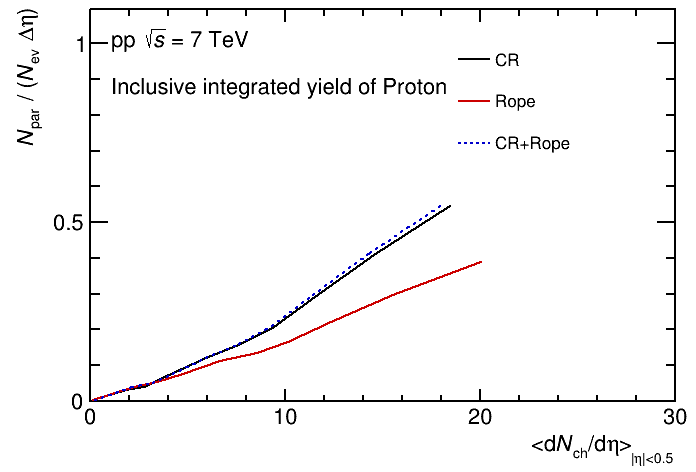
\includegraphics[width=.48\textwidth]{Proton_InteSpectrum}
	\end{center}
	\caption{Inclusive integrated yields of particles with $\avdndeta$.(Data taken from arXiv:1606.07424v2 and arXiv:1910.14397v1)}
	\label{fig:InclIntePar}
\end{figure}
%===================================================================
\begin{figure}[ht]
	\begin{center}
		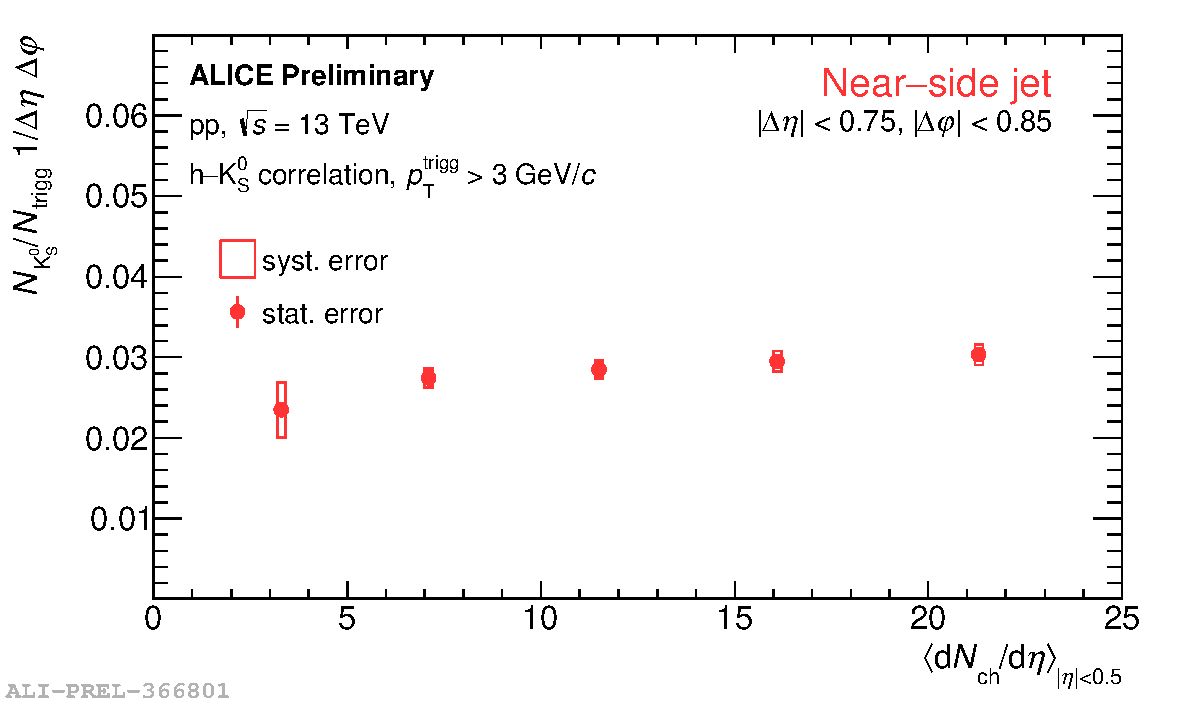
\includegraphics[width=.48\textwidth]{FinalYieldvsMultK0sJet_0}
		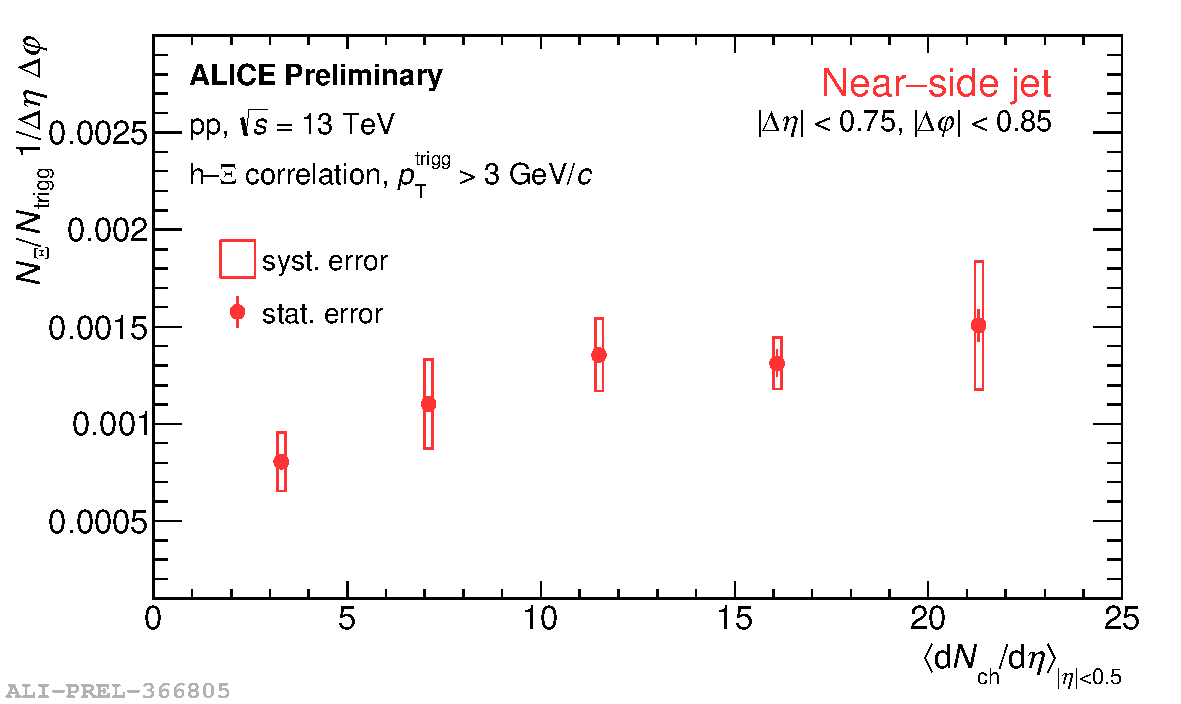
\includegraphics[width=.48\textwidth]{FinalYieldvsMultXiJet_0}
		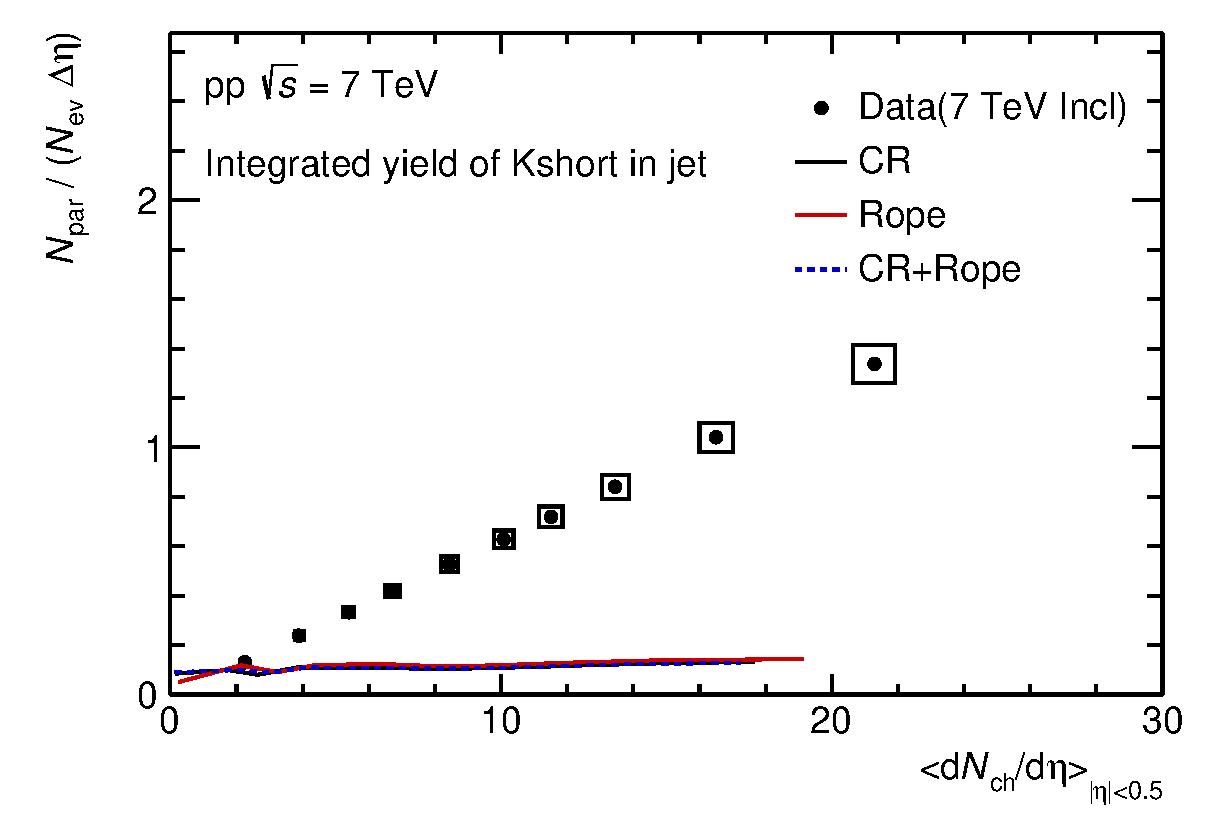
\includegraphics[width=.48\textwidth]{Kshort_InteSpectrum_JE}
		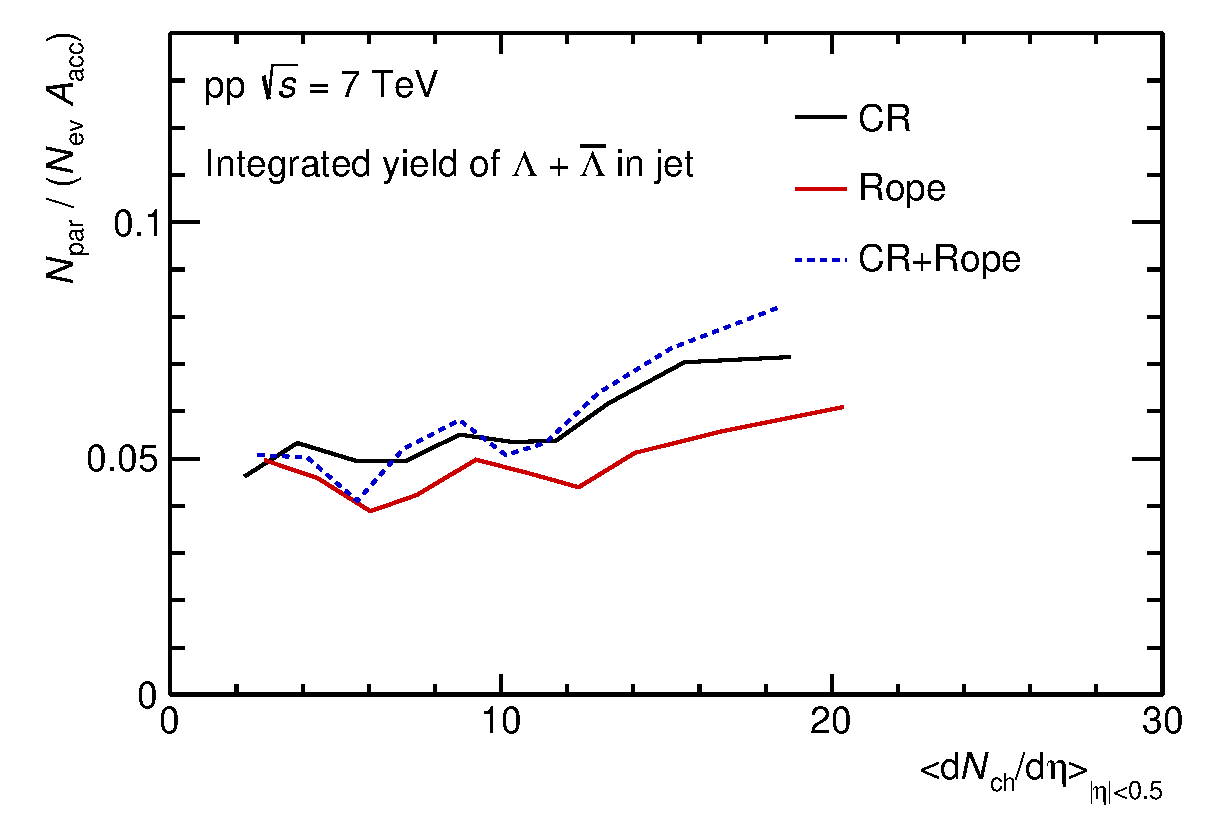
\includegraphics[width=.48\textwidth]{Lambda_InteSpectrum_JE}
		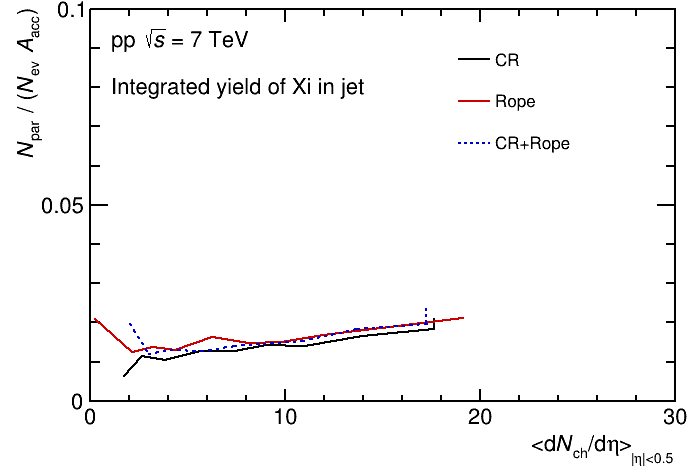
\includegraphics[width=.48\textwidth]{Xi_InteSpectrum_JE}
		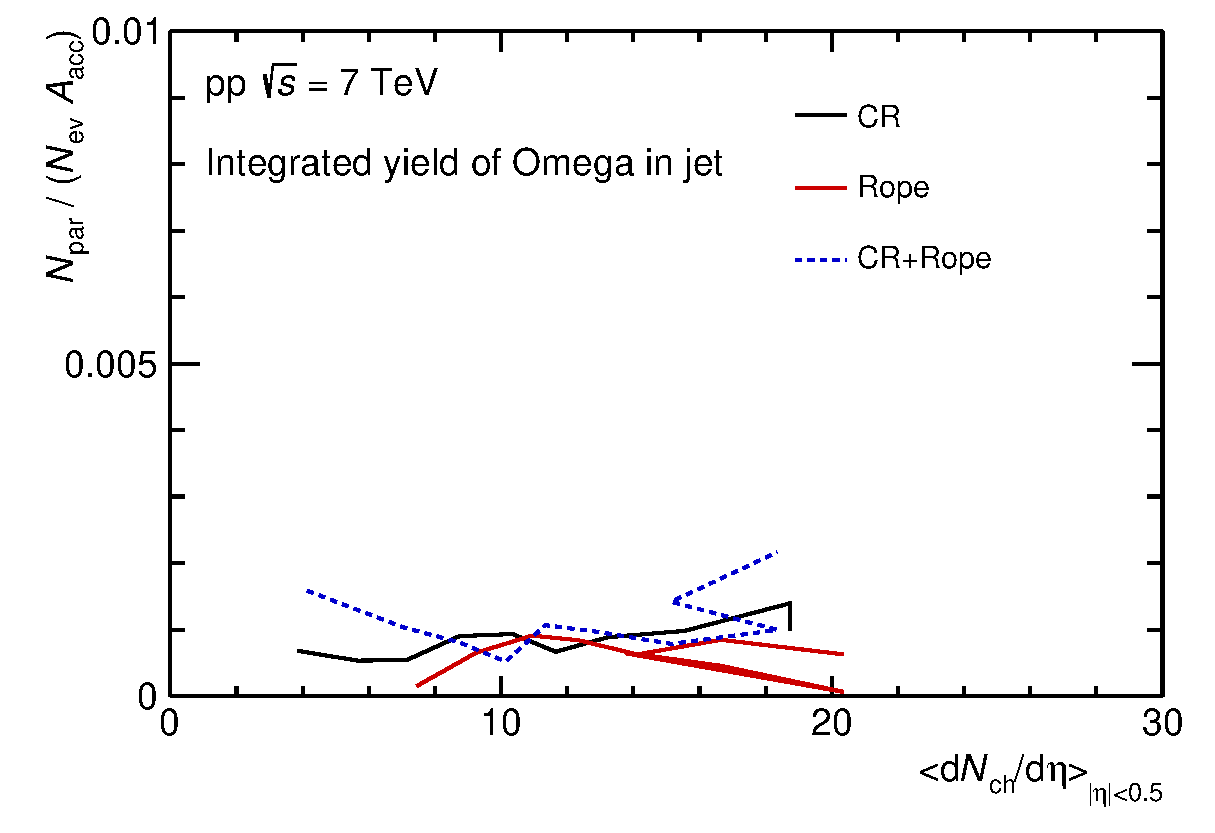
\includegraphics[width=.48\textwidth]{Omega_InteSpectrum_JE}
		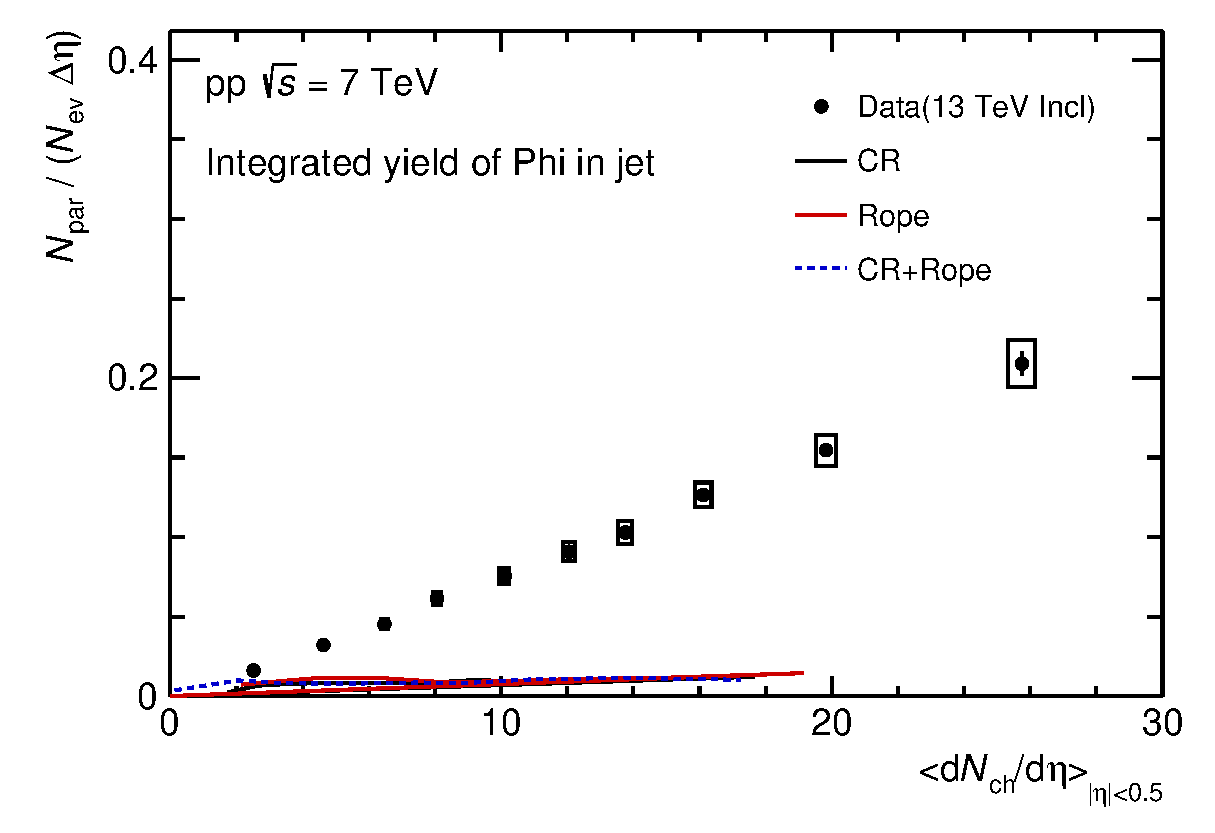
\includegraphics[width=.48\textwidth]{Phi_InteSpectrum_JE}
		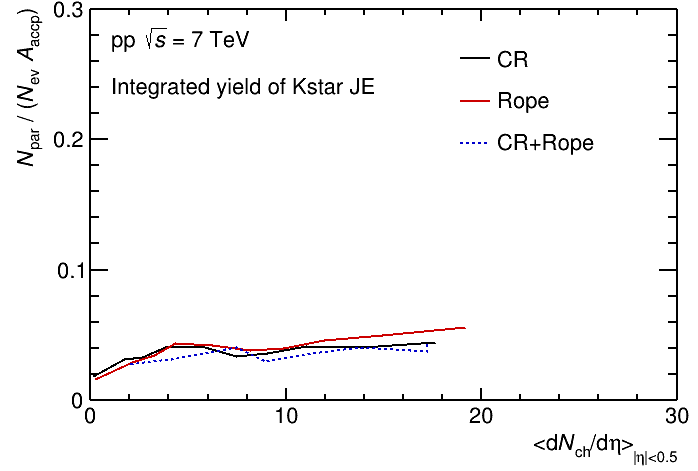
\includegraphics[width=.48\textwidth]{Kstar_InteSpectrum_JE}
	\end{center}
	\caption{Integrated yields of particles in jet with $\avdndeta$.(Data point at 13 TeV is used hadron-strange correlation method)}
	\label{fig:JCIntePar}
\end{figure}

%===================================================================
\begin{figure}[ht]
	\begin{center}
		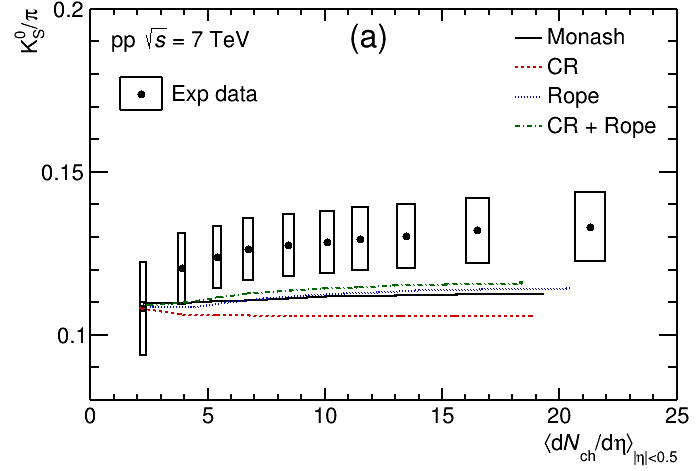
\includegraphics[width=.48\textwidth]{Kshort_PiRatio}
		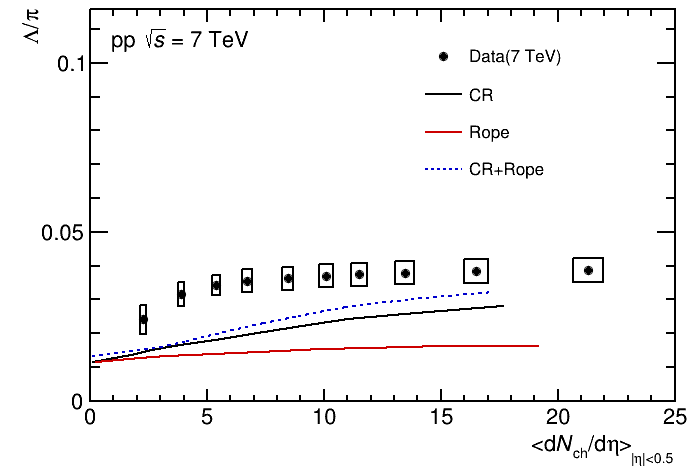
\includegraphics[width=.48\textwidth]{Lambda_PiRatio}
		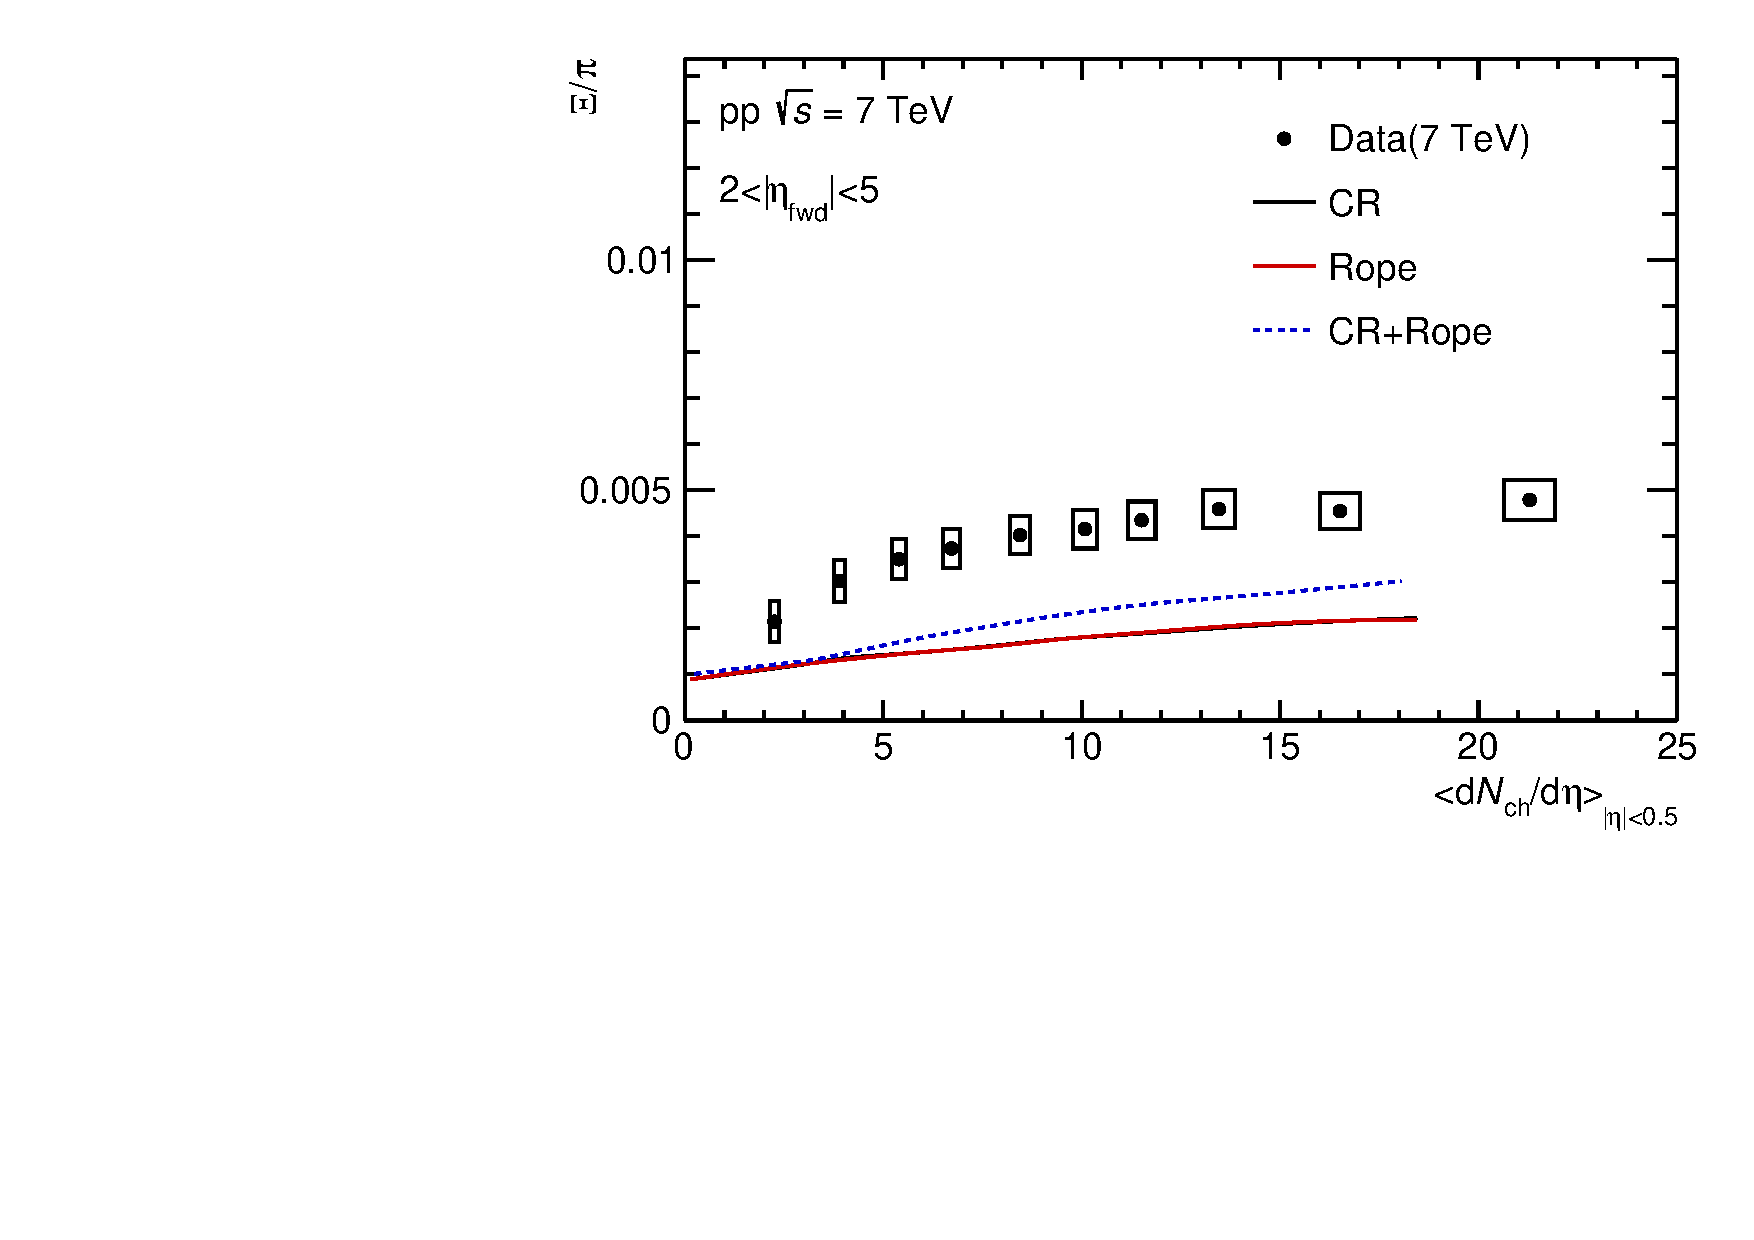
\includegraphics[width=.48\textwidth]{Xi_PiRatio}
		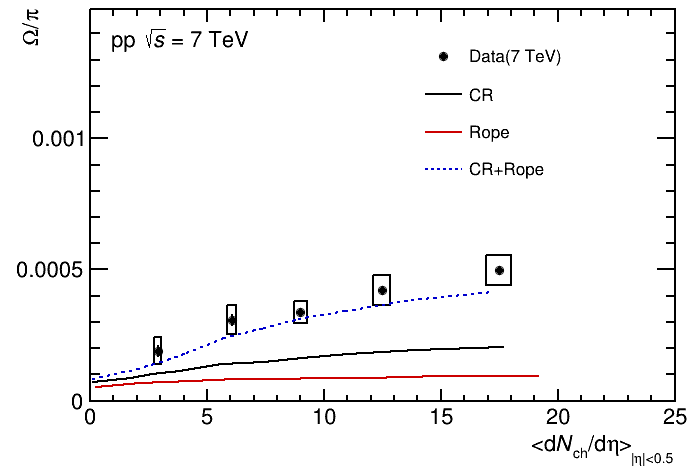
\includegraphics[width=.48\textwidth]{Omega_PiRatio}
		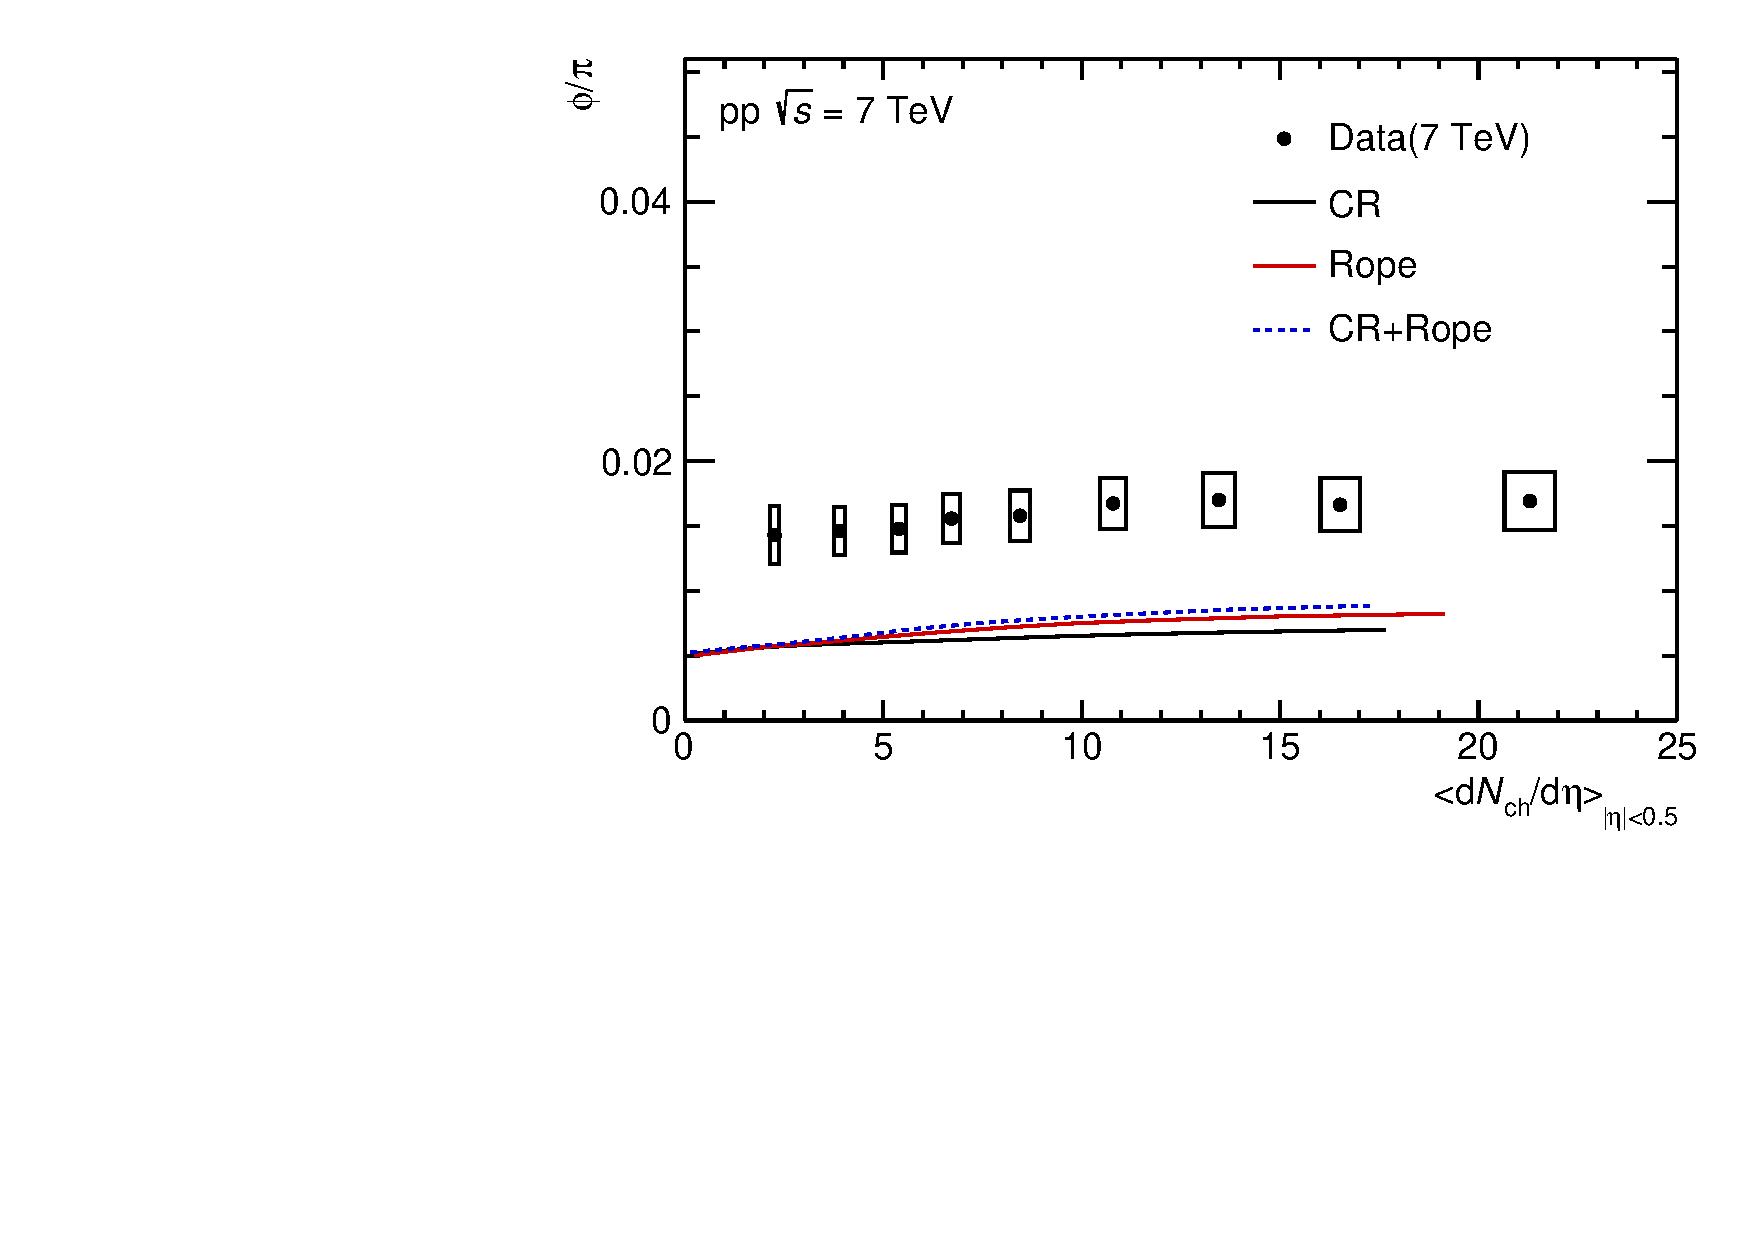
\includegraphics[width=.48\textwidth]{Phi_PiRatio}	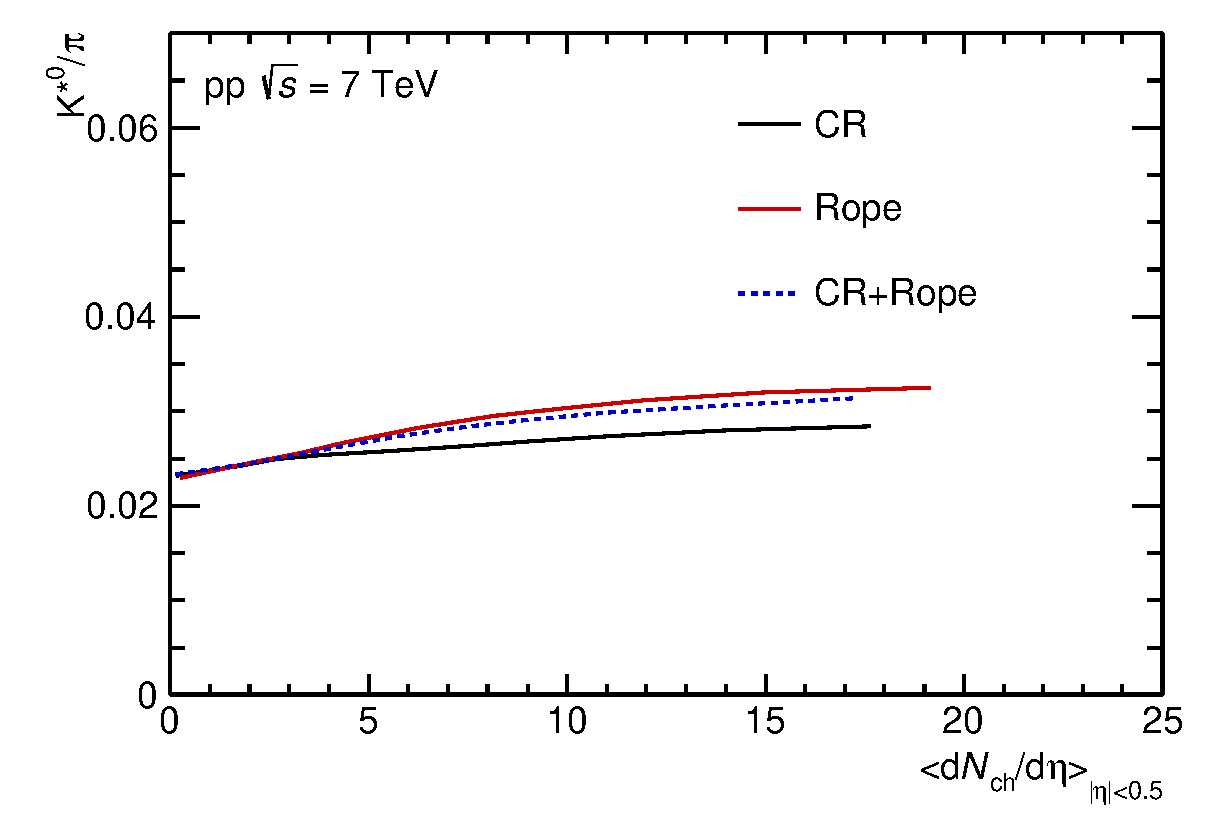
\includegraphics[width=.48\textwidth]{Kstar_PiRatio}
	\end{center}
	\caption{Inclusive integrated yields ratios of strange particle to $\pi$ with $\avdndeta$. (Data taken from arXiv:1606.07424v2 and arXiv:1807.11321v2)}
	\label{fig:InclIntePartoPiRatio}
\end{figure}


%===================================================================
\begin{figure}[ht]
	\begin{center}
		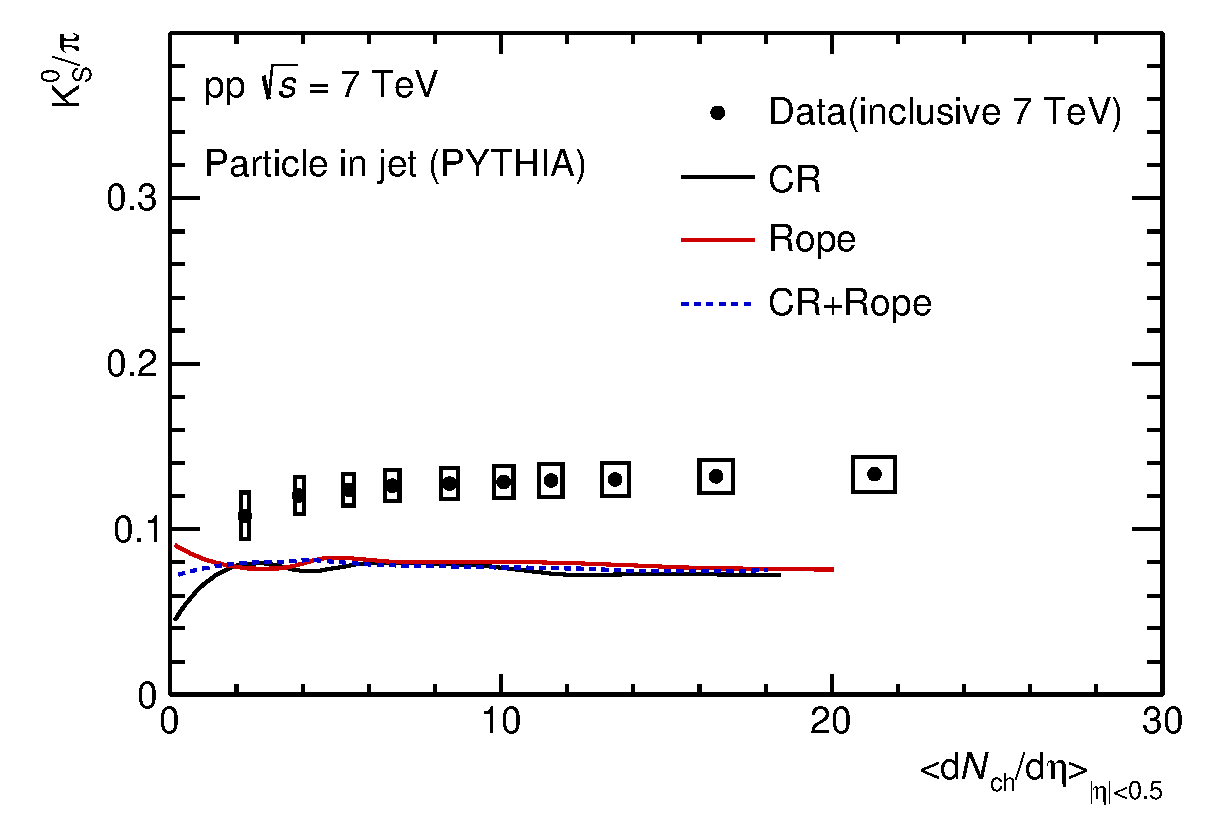
\includegraphics[width=.48\textwidth]{Kshort_PiRatio_JE}
		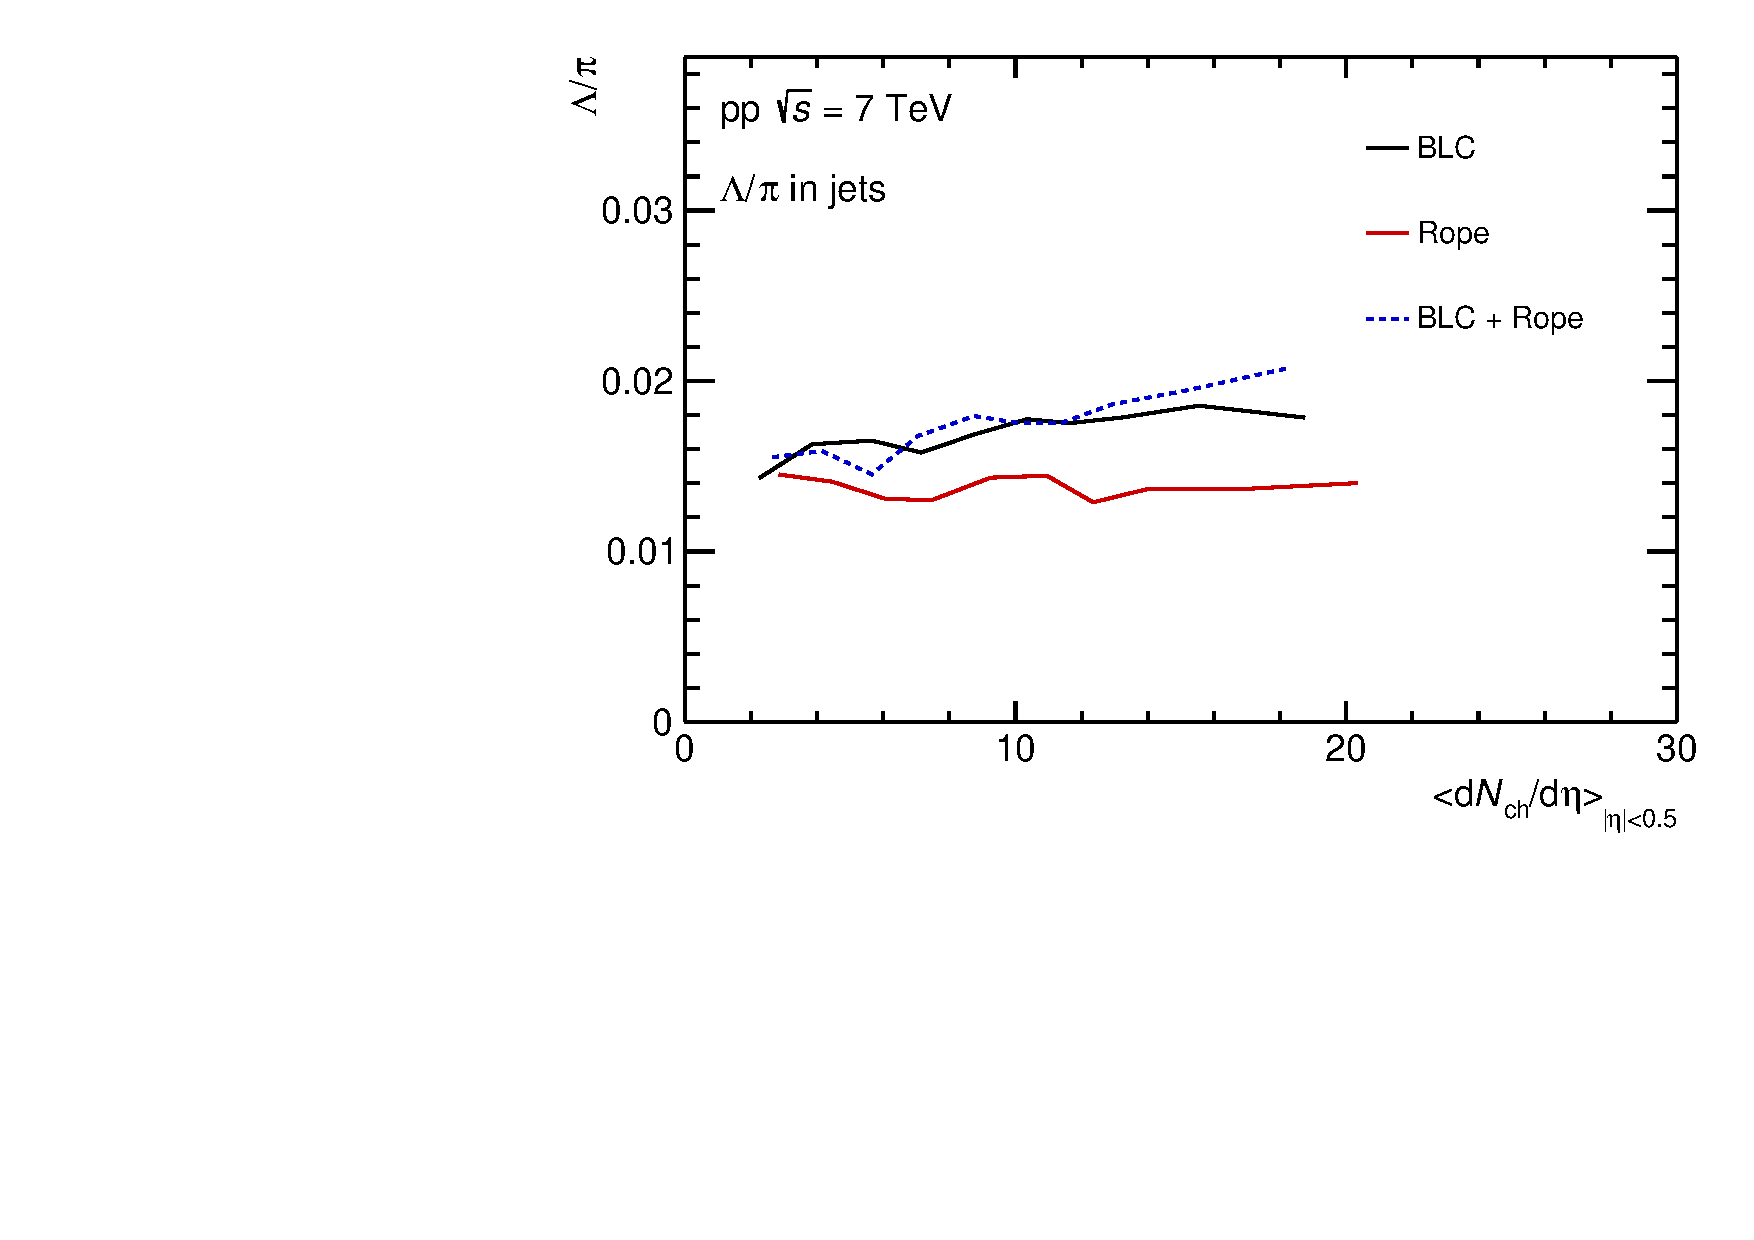
\includegraphics[width=.48\textwidth]{Lambda_PiRatio_JE}
		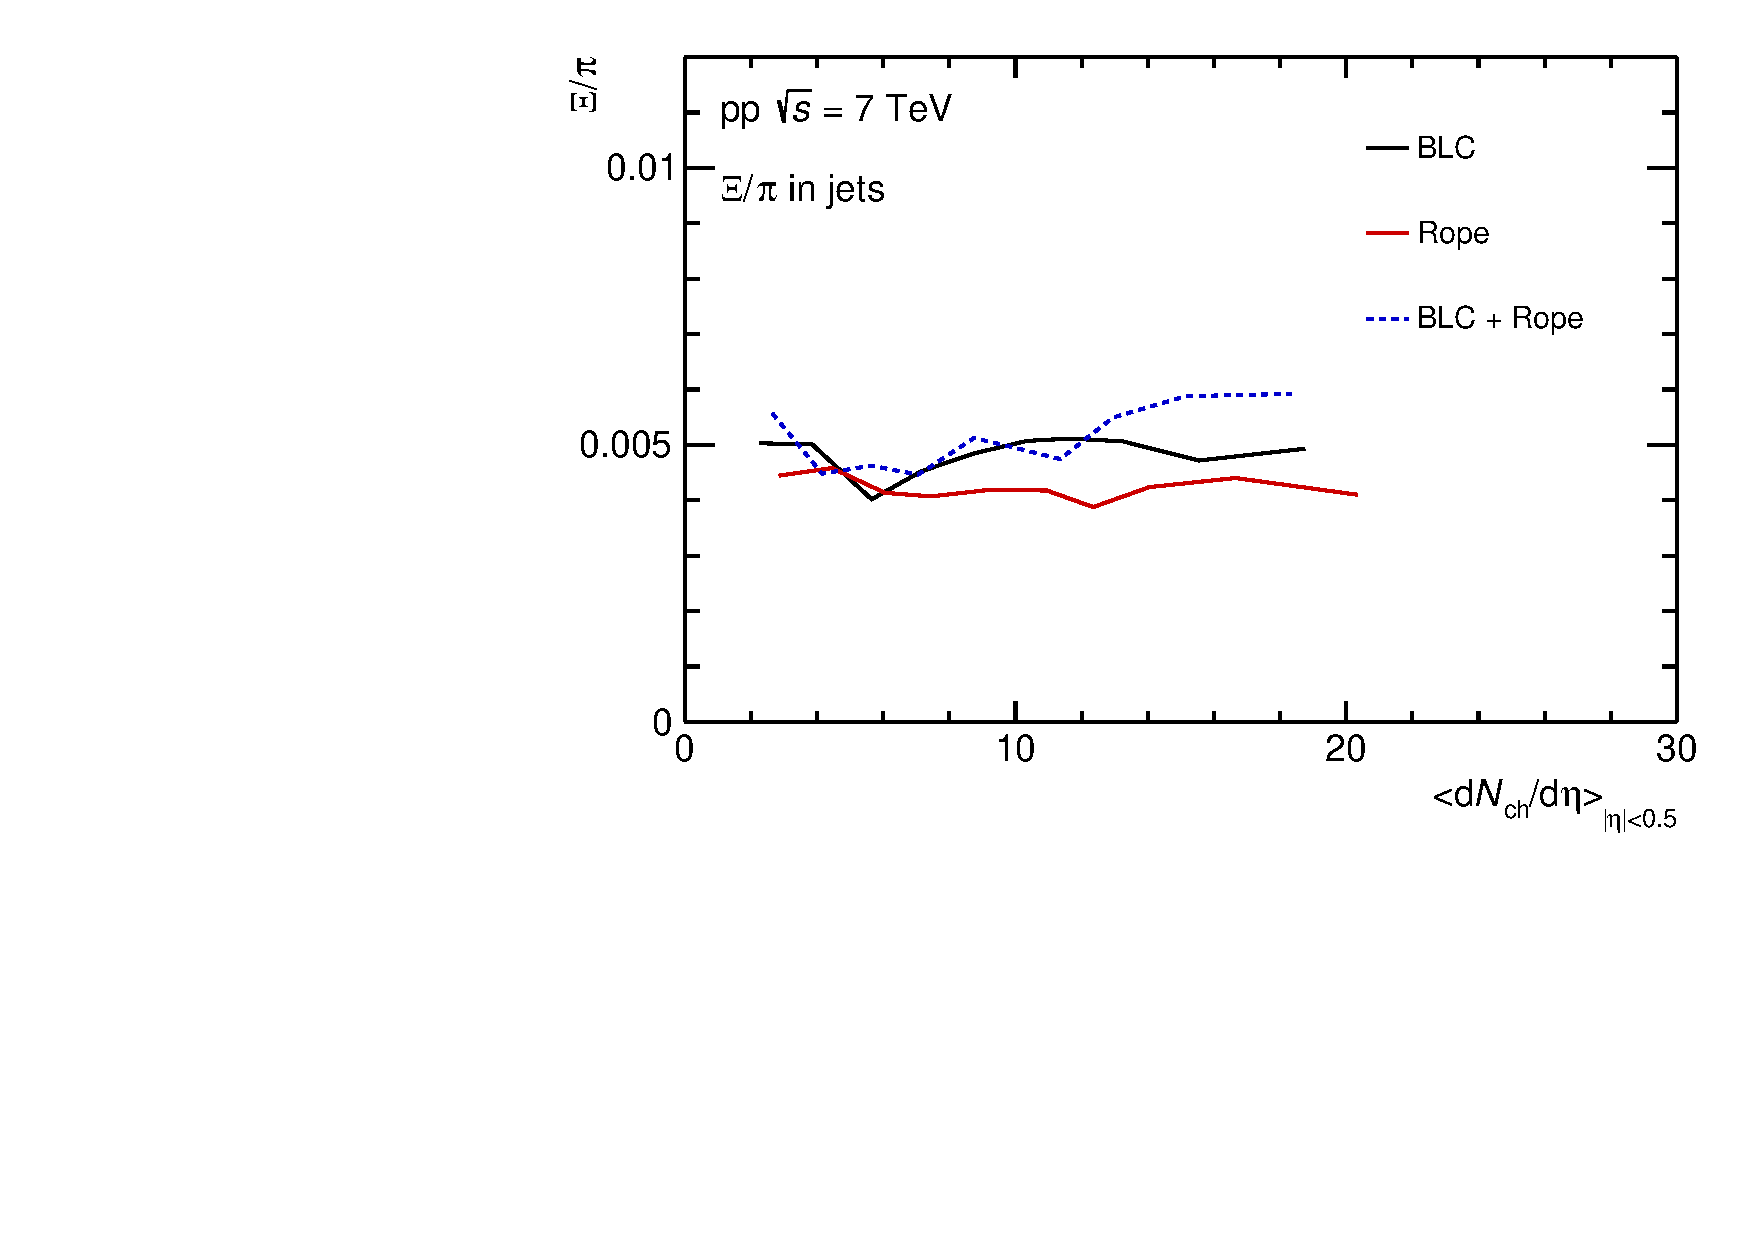
\includegraphics[width=.48\textwidth]{Xi_PiRatio_JE}
		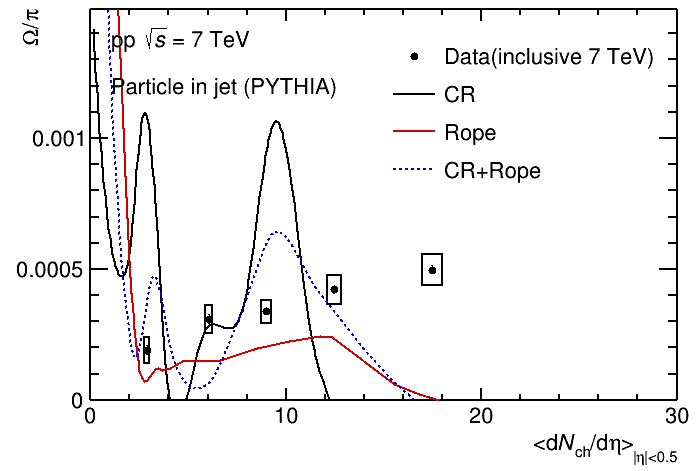
\includegraphics[width=.48\textwidth]{Omega_PiRatio_JE}
		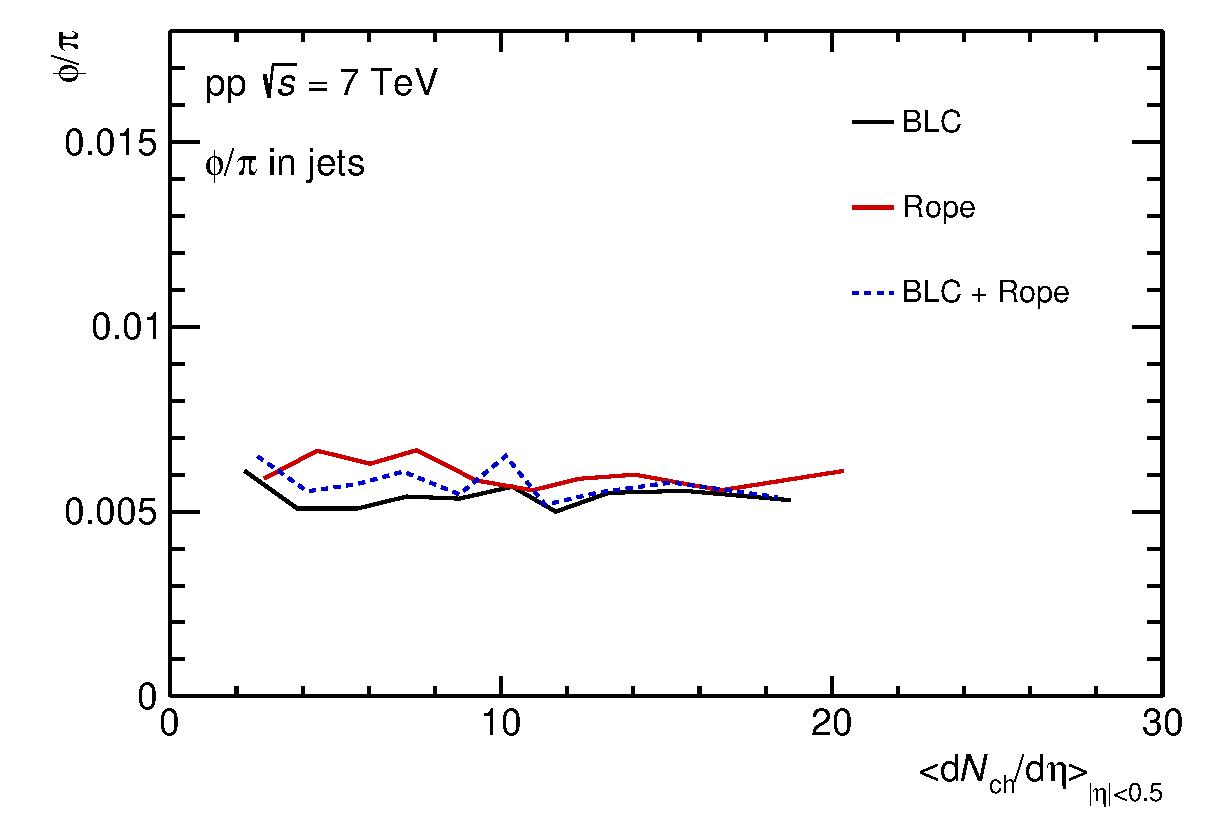
\includegraphics[width=.48\textwidth]{Phi_PiRatio_JE}
		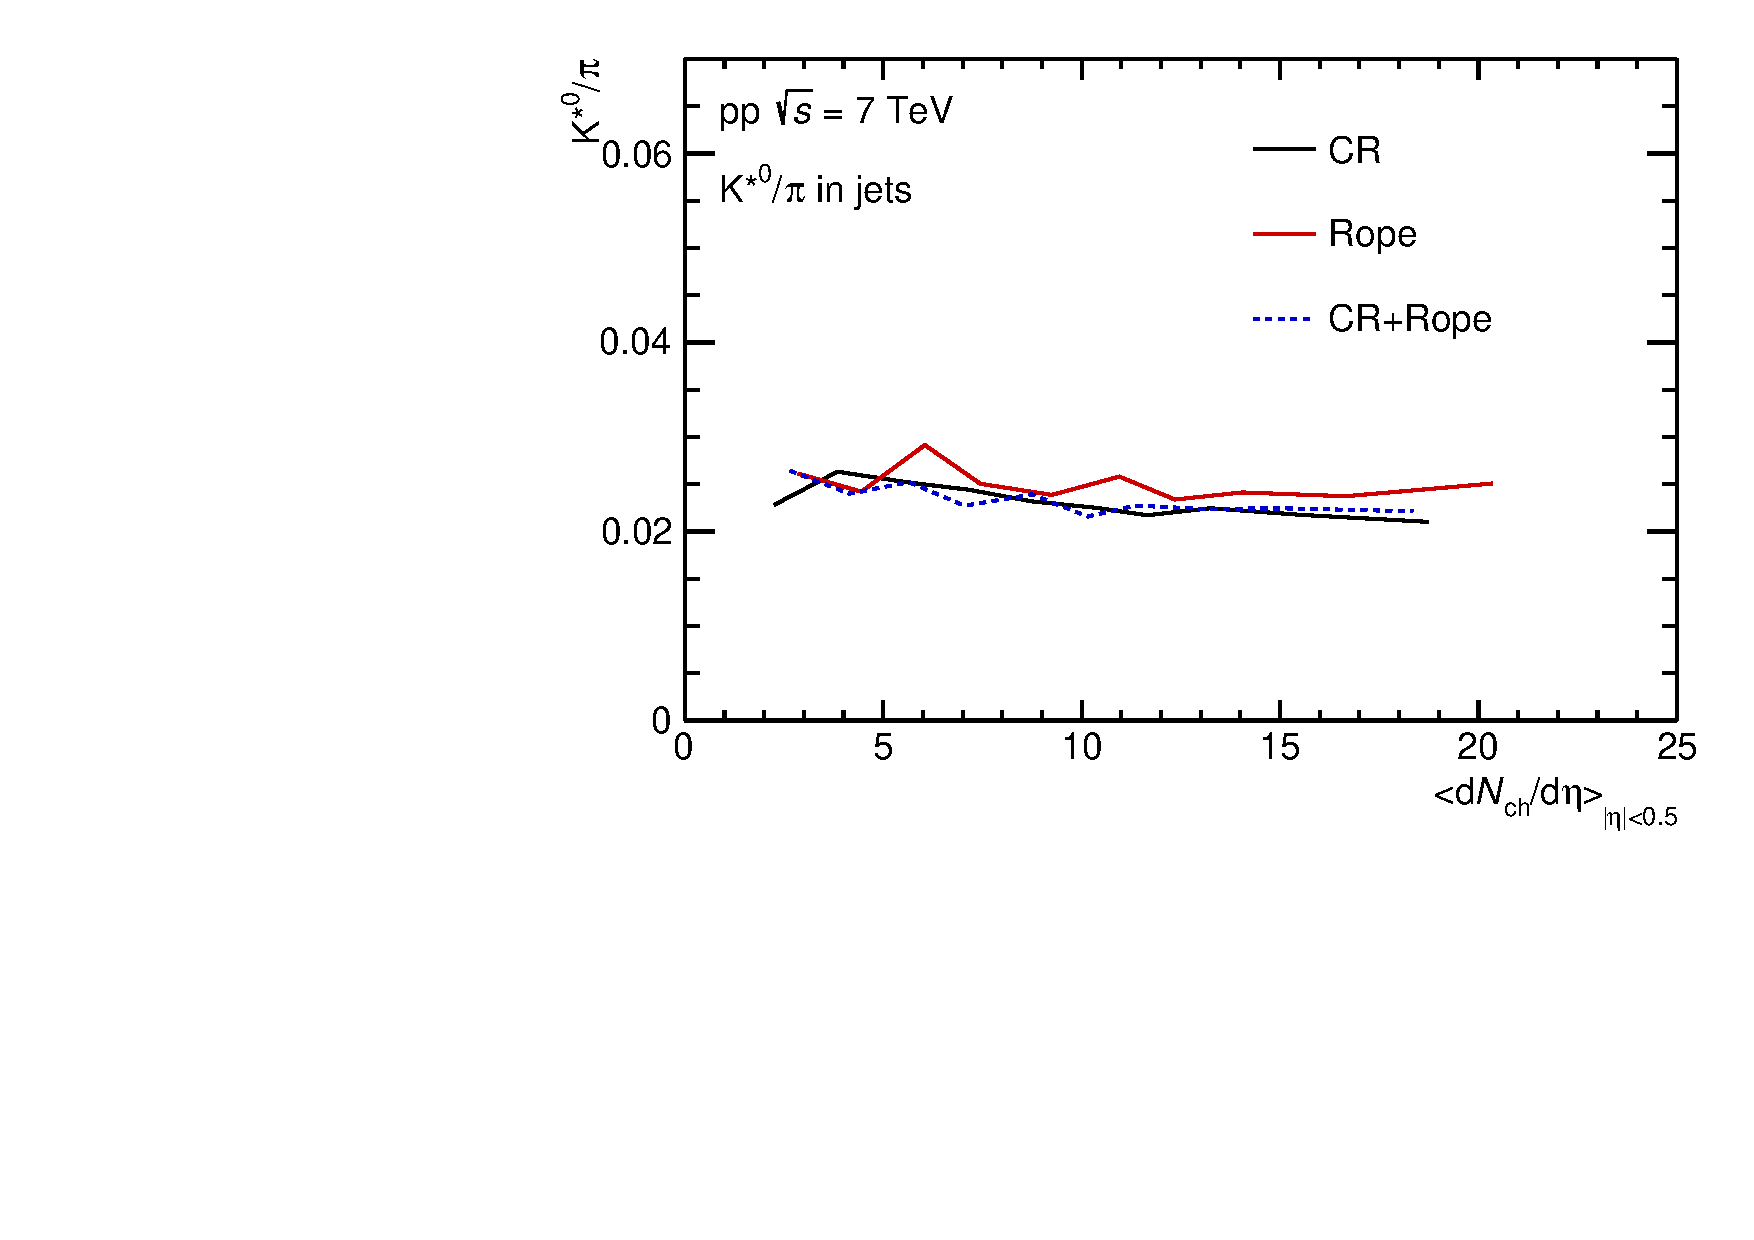
\includegraphics[width=.48\textwidth]{Kstar_PiRatio_JE}
	\end{center}
	\caption{Integrated yields ratios in jet of strange particle to $\pi$ with $\avdndeta$. (Data taken from arXiv:1606.07424v2 and arXiv:1807.11321v2)}
	\label{fig:JEIntePartoPiRatio}
\end{figure}

\begin{figure}[ht]
	\begin{center}
				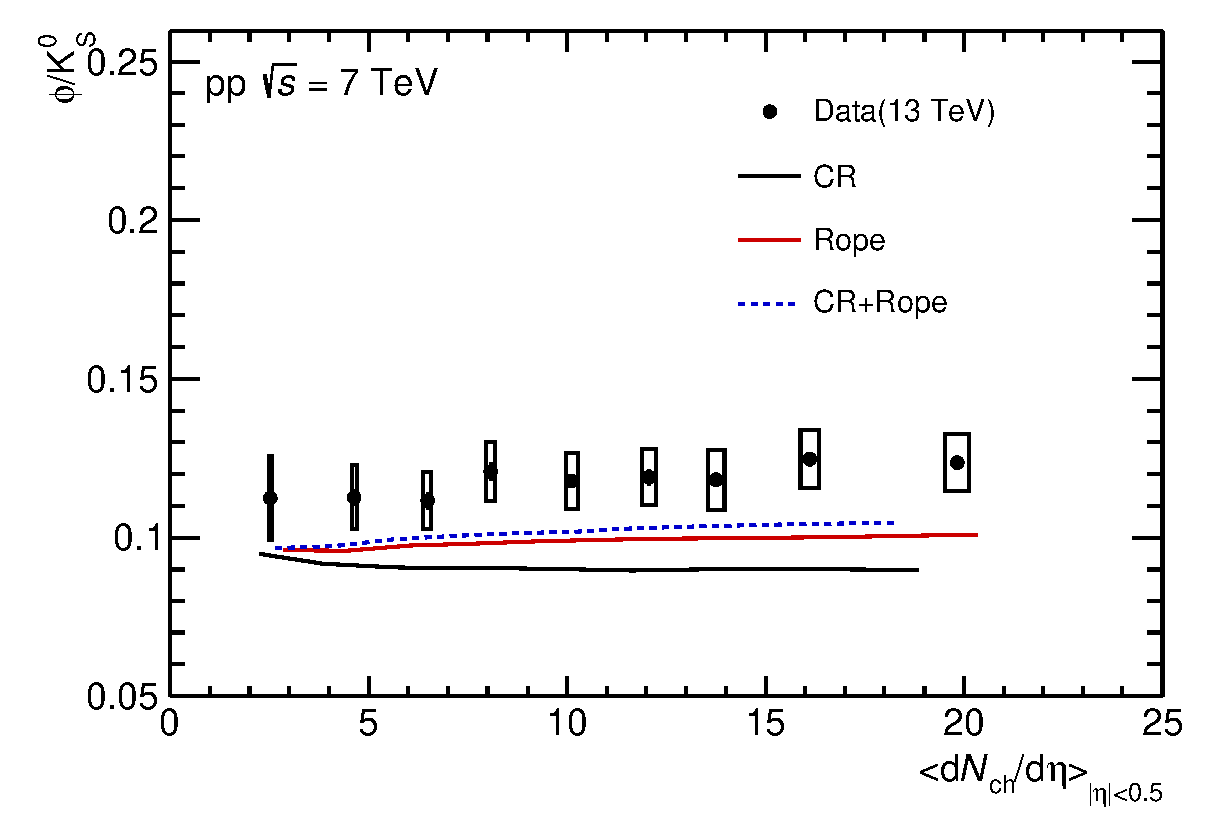
\includegraphics[width=.48\textwidth]{Inte_PhiKRatio}		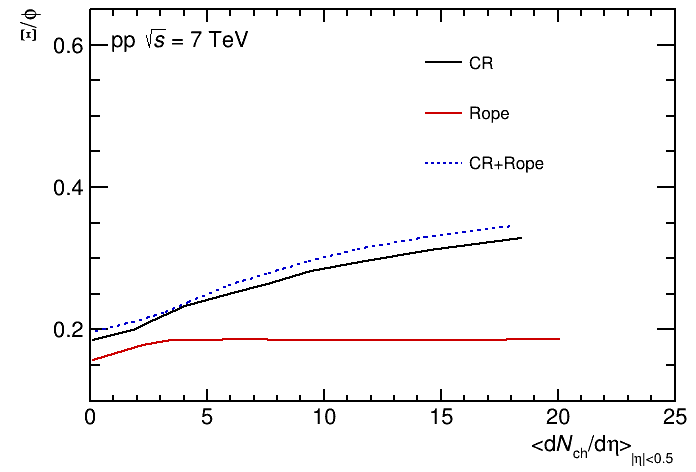
\includegraphics[width=.48\textwidth]{Inte_XiPhiRatio}
		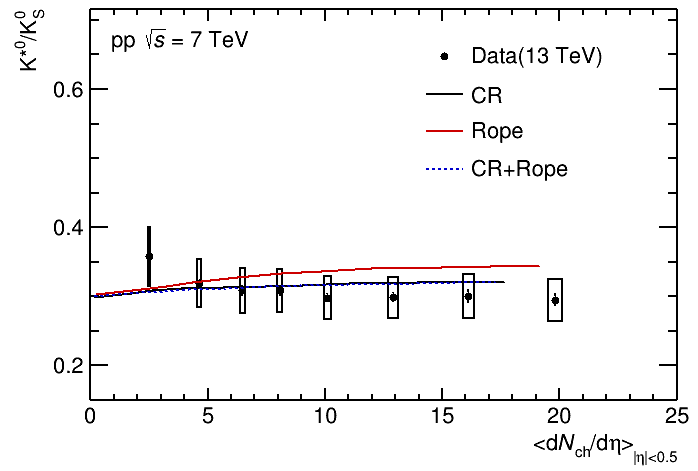
\includegraphics[width=.48\textwidth]{Inte_KstarKRatio}
		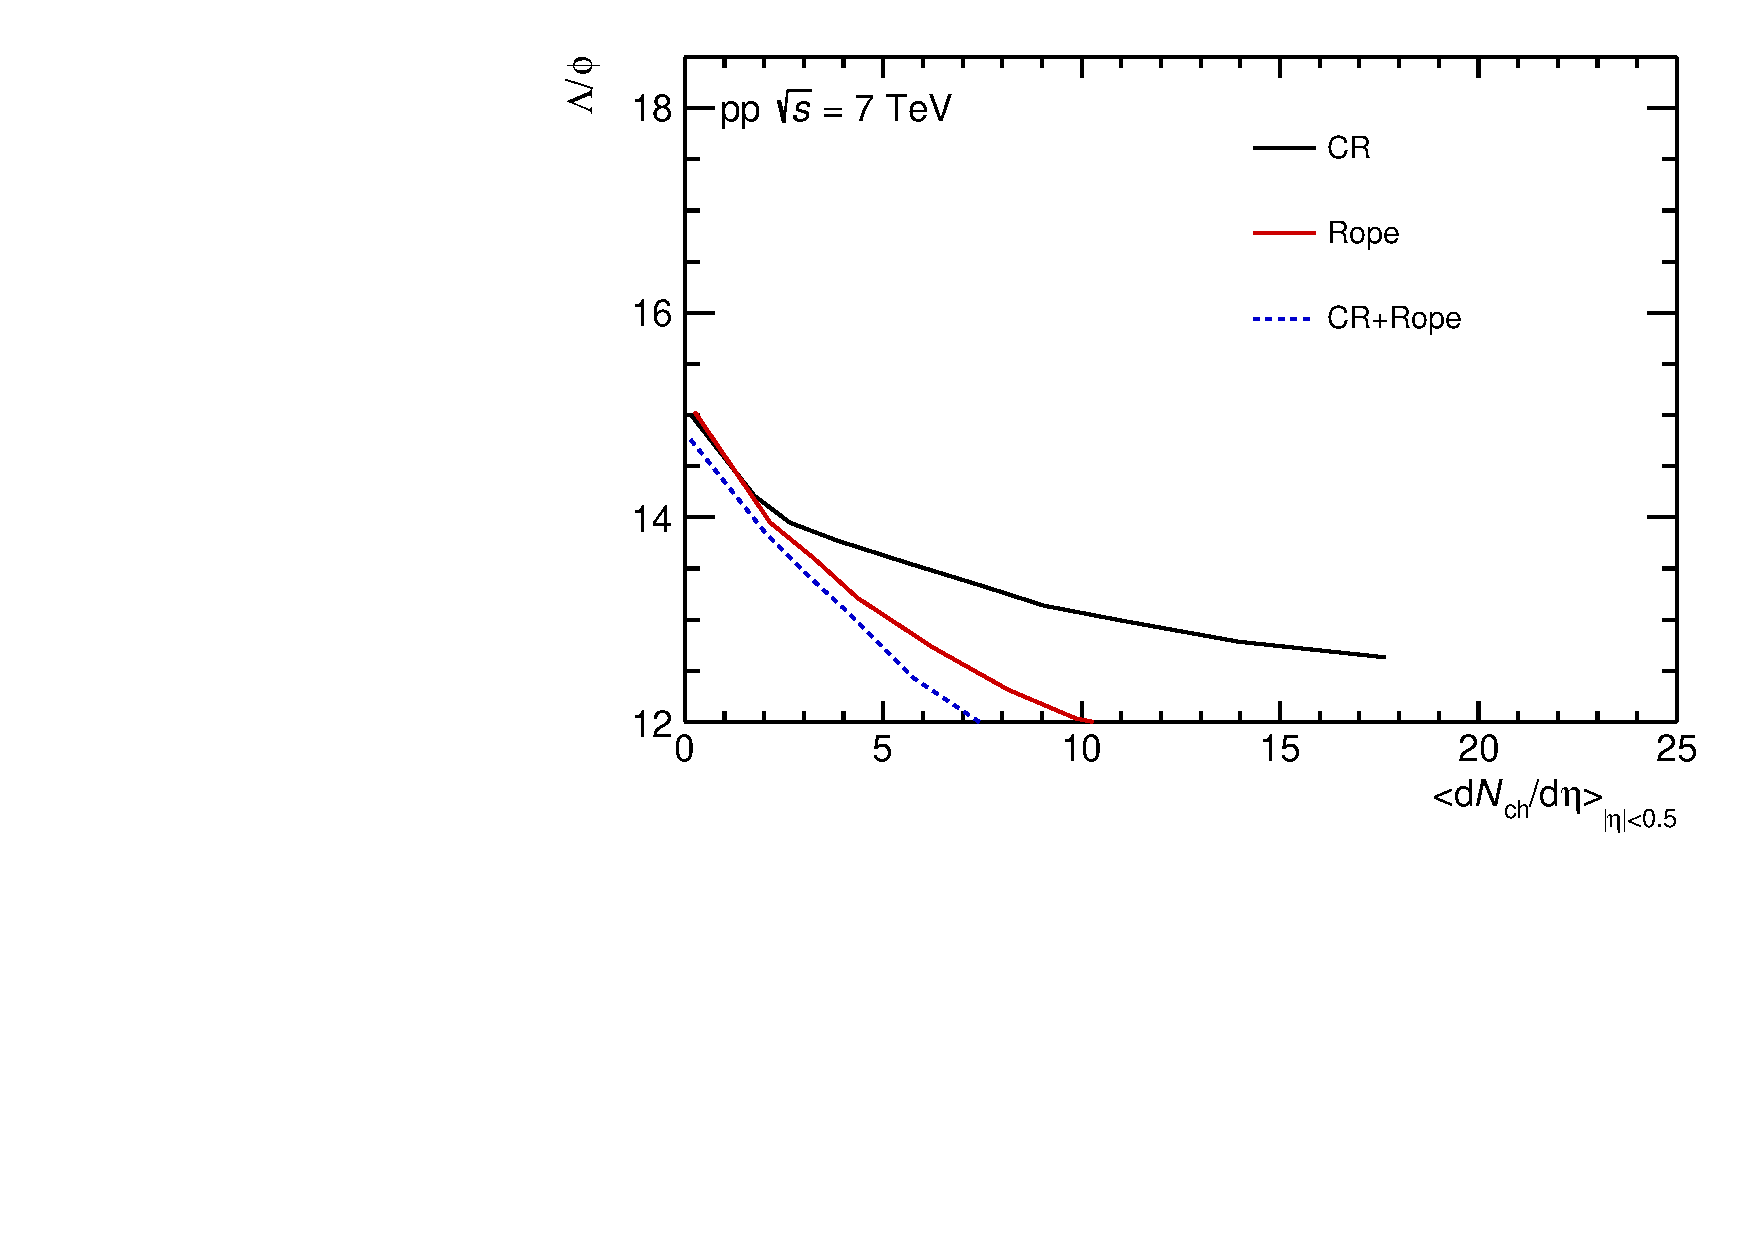
\includegraphics[width=.48\textwidth]{Inte_LambdaPhiRatio}
		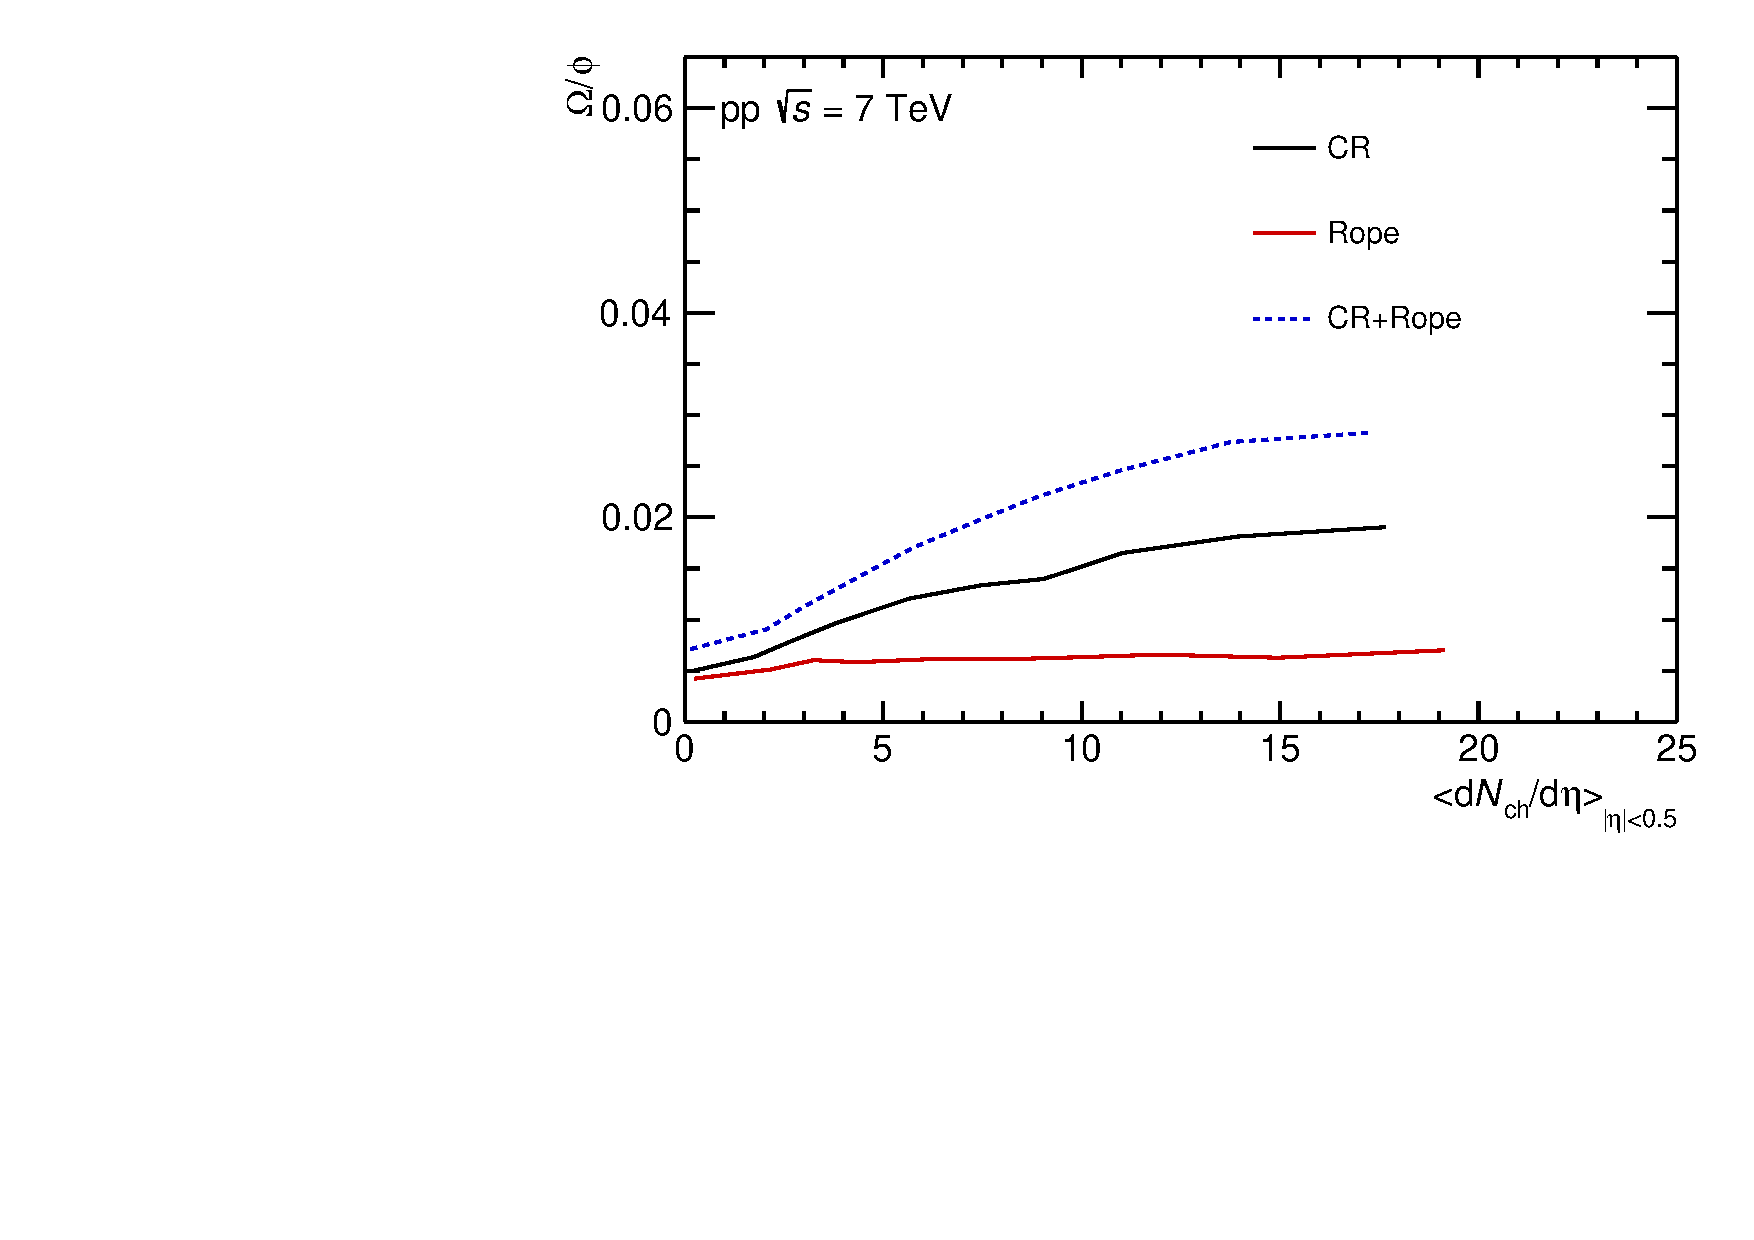
\includegraphics[width=.48\textwidth]{Inte_OmegaPhiRatio}
		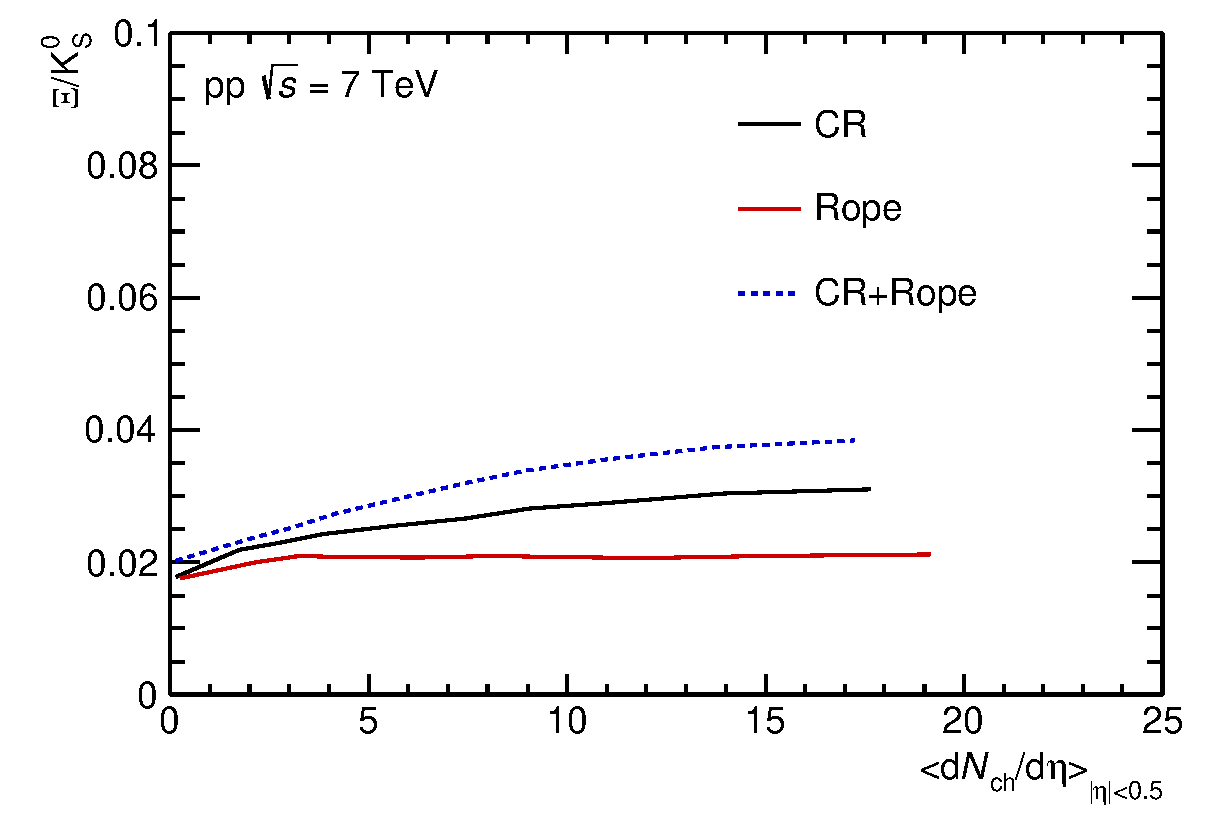
\includegraphics[width=.48\textwidth]{Inte_XiKshortRatio}
		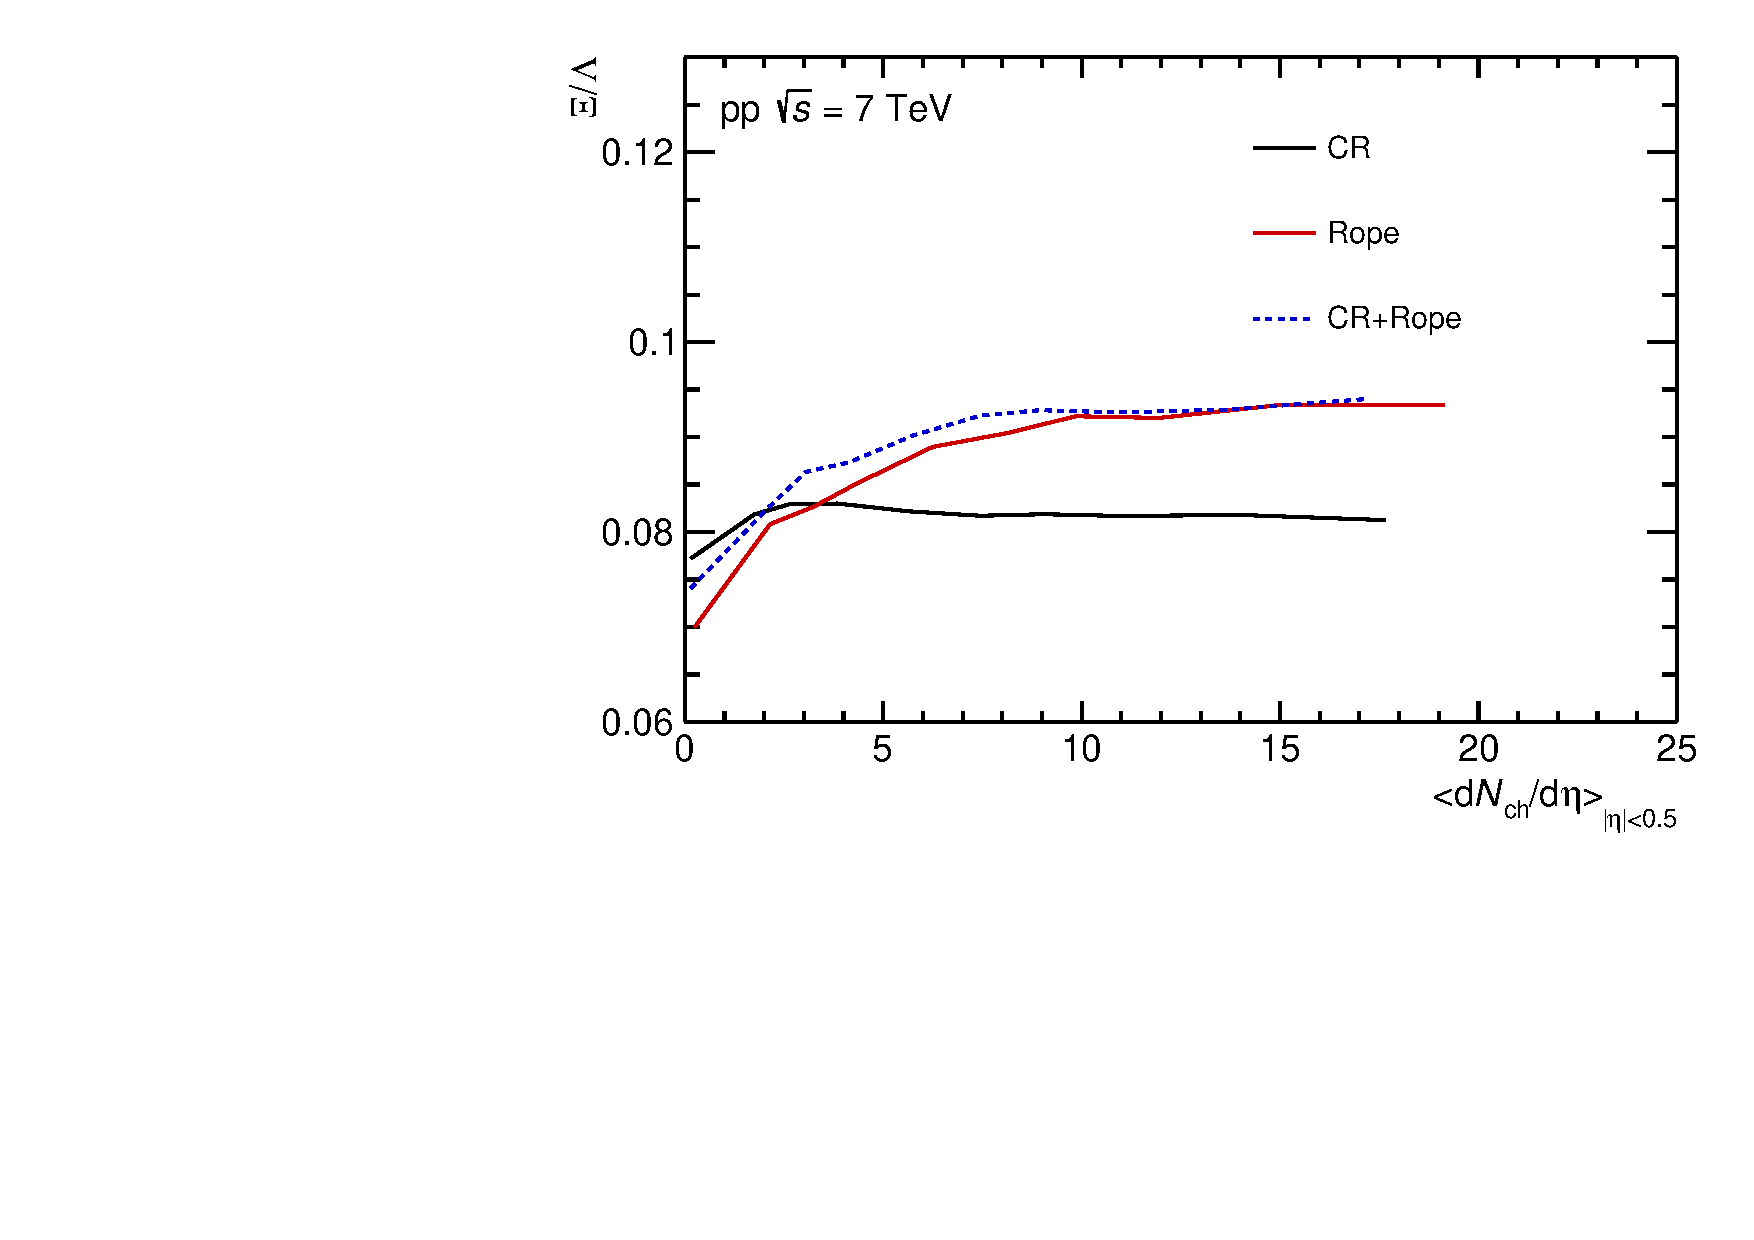
\includegraphics[width=.48\textwidth]{Inte_XiLambdaRatio}
		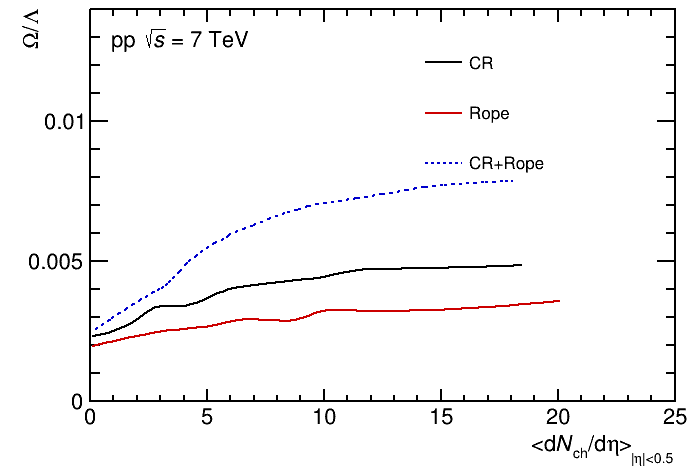
\includegraphics[width=.48\textwidth]{Inte_OmegaLambdaRatio}
	\end{center}
	\caption{Inclusive integrated yields ratios with $\avdndeta$.(Data taken from arXiv:1910.14397v1)}
	\label{fig:InclInteParRatio}
\end{figure}

\begin{figure}[ht]
	\begin{center}	
		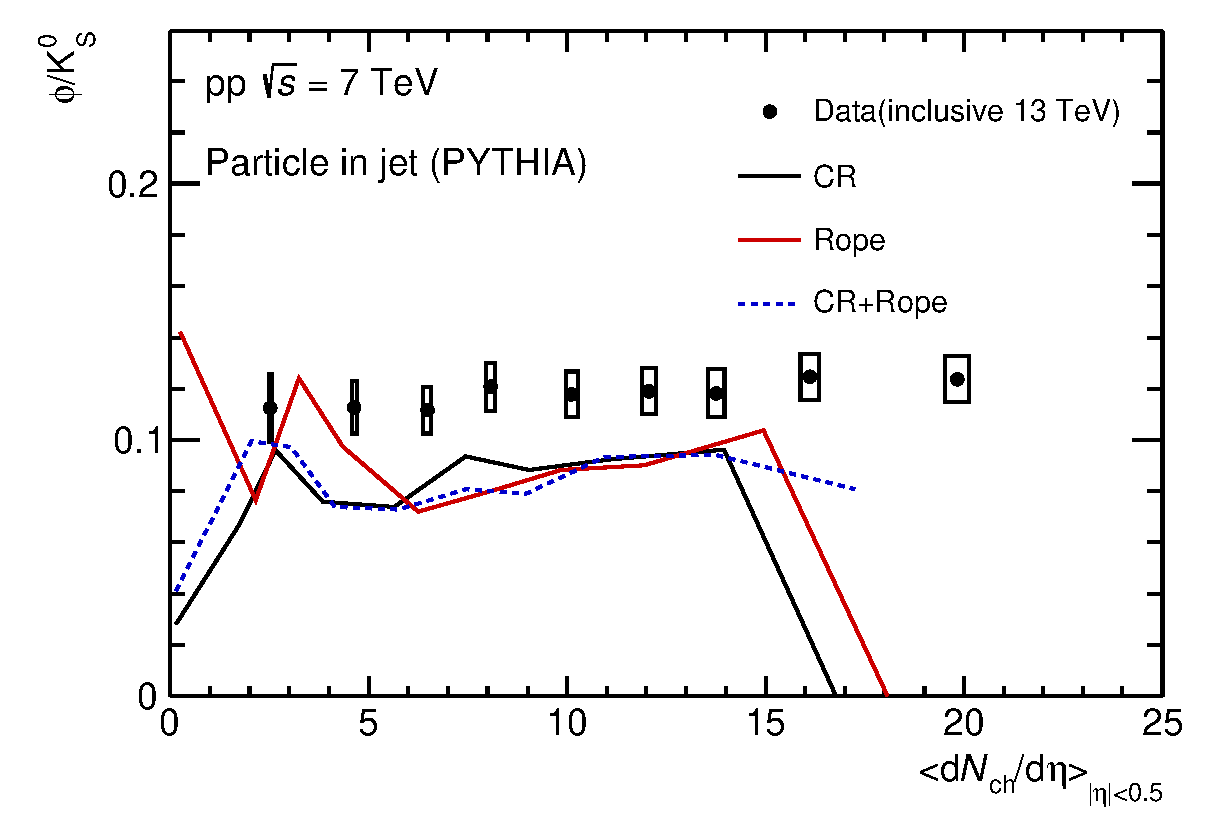
\includegraphics[width=.48\textwidth]{Inte_PhiKRatio_JE}		
		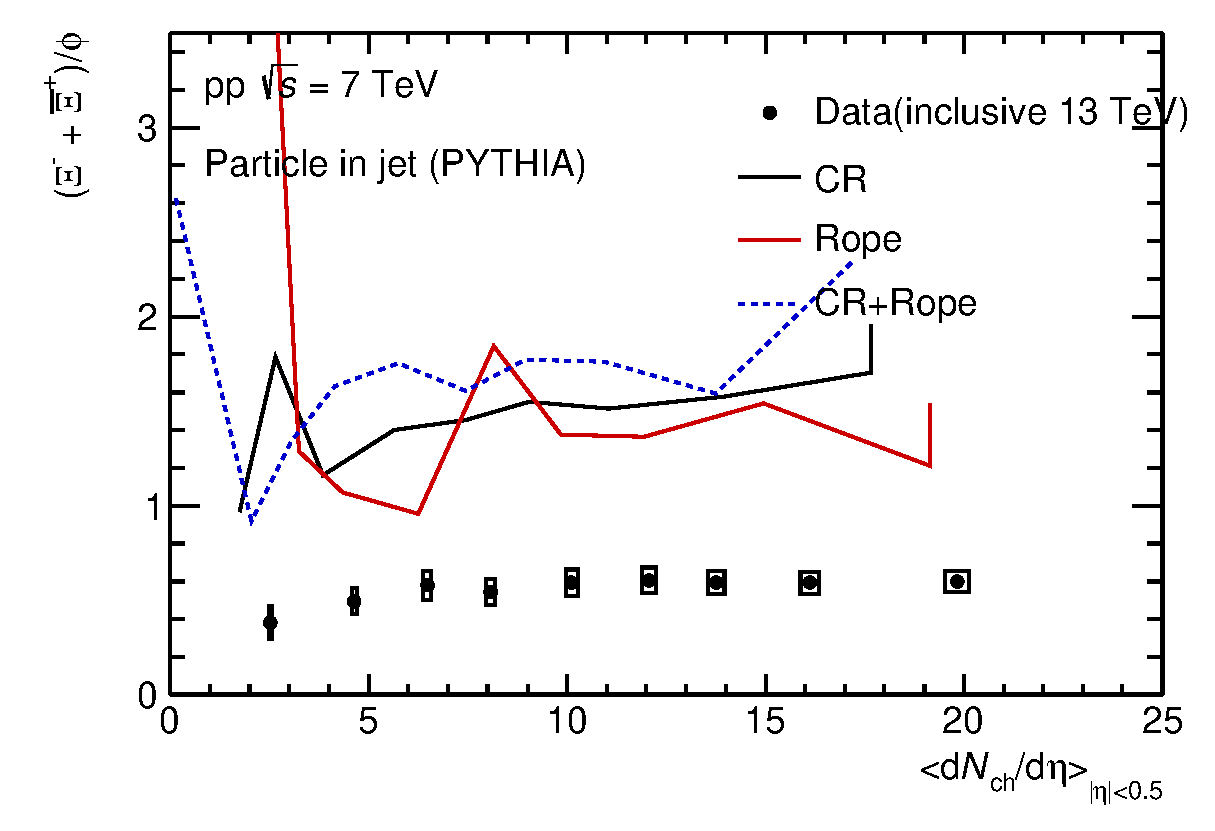
\includegraphics[width=.48\textwidth]{Inte_XiPhiRatio_JE}
		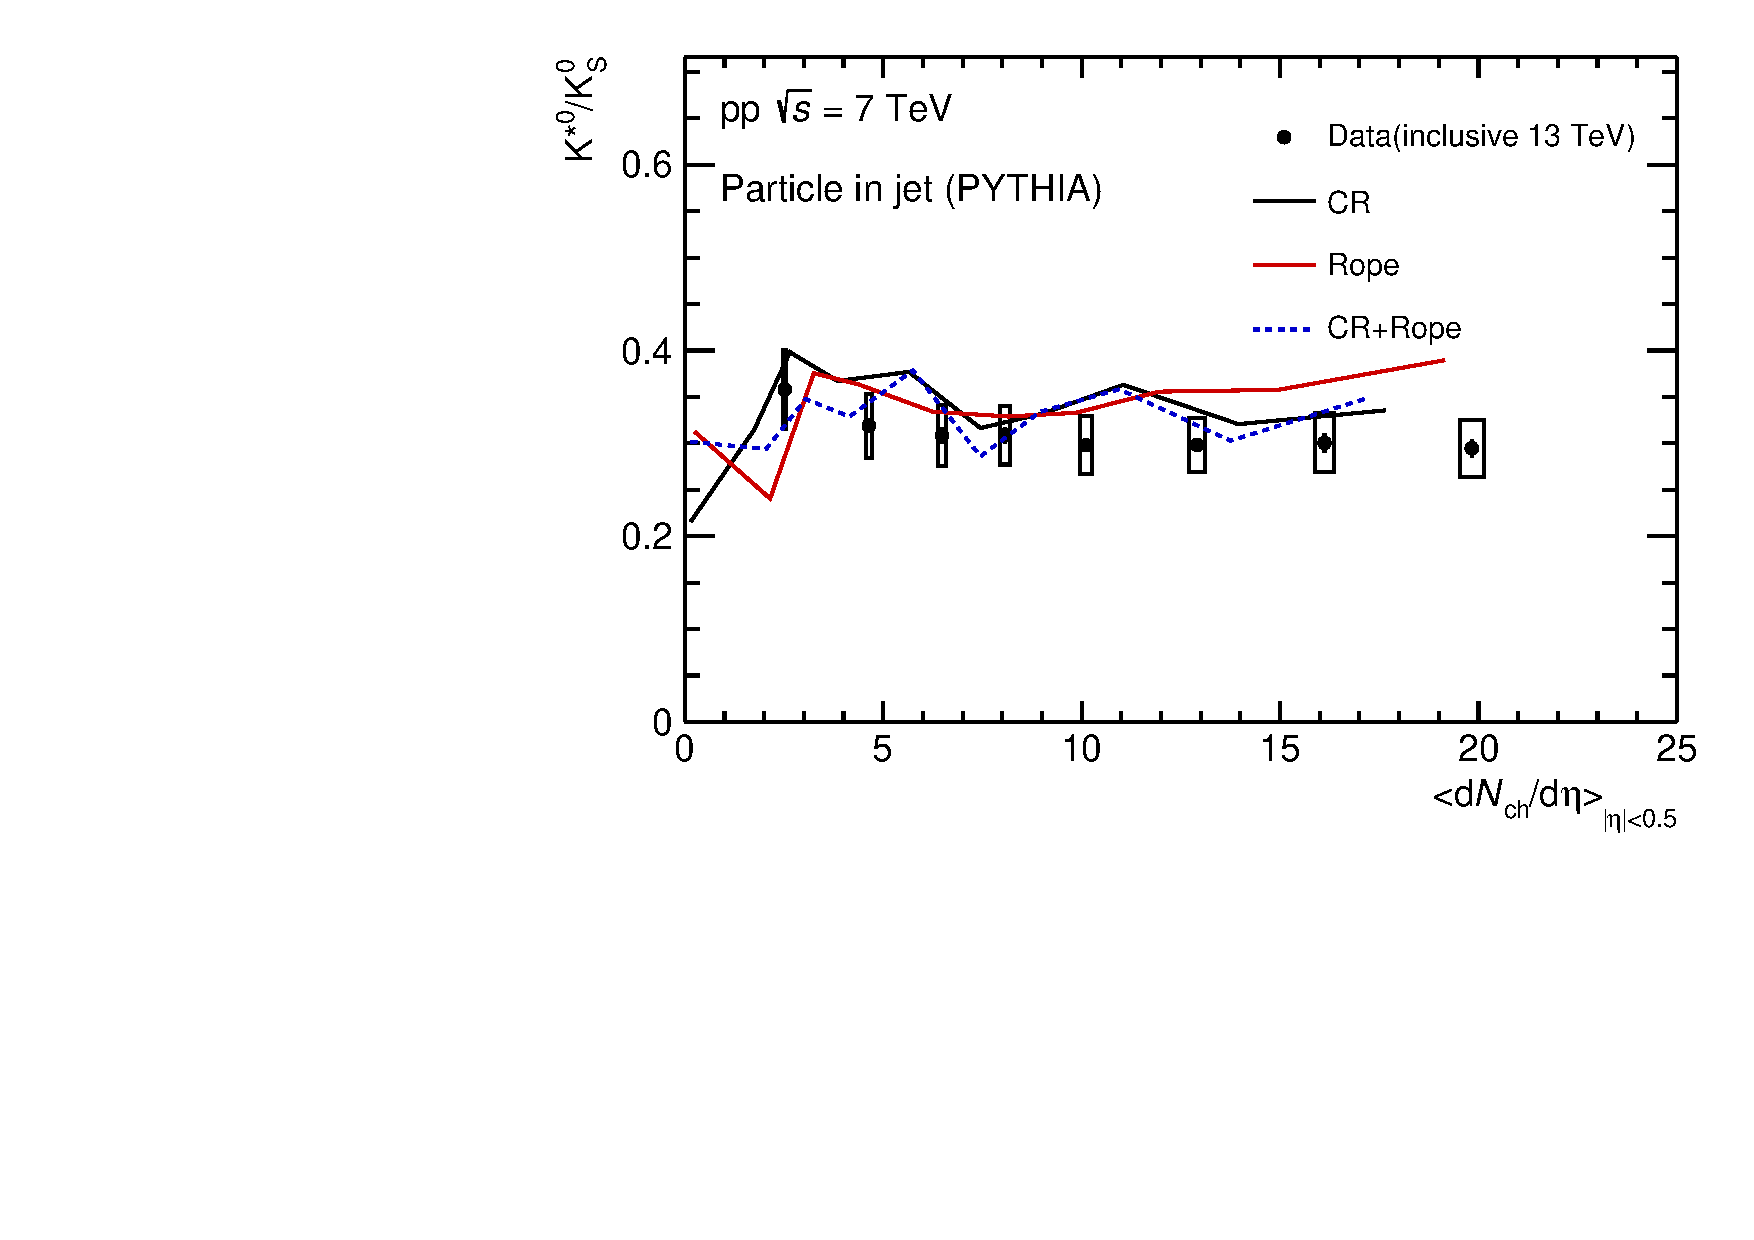
\includegraphics[width=.48\textwidth]{Inte_KstarKRatio_JE}
		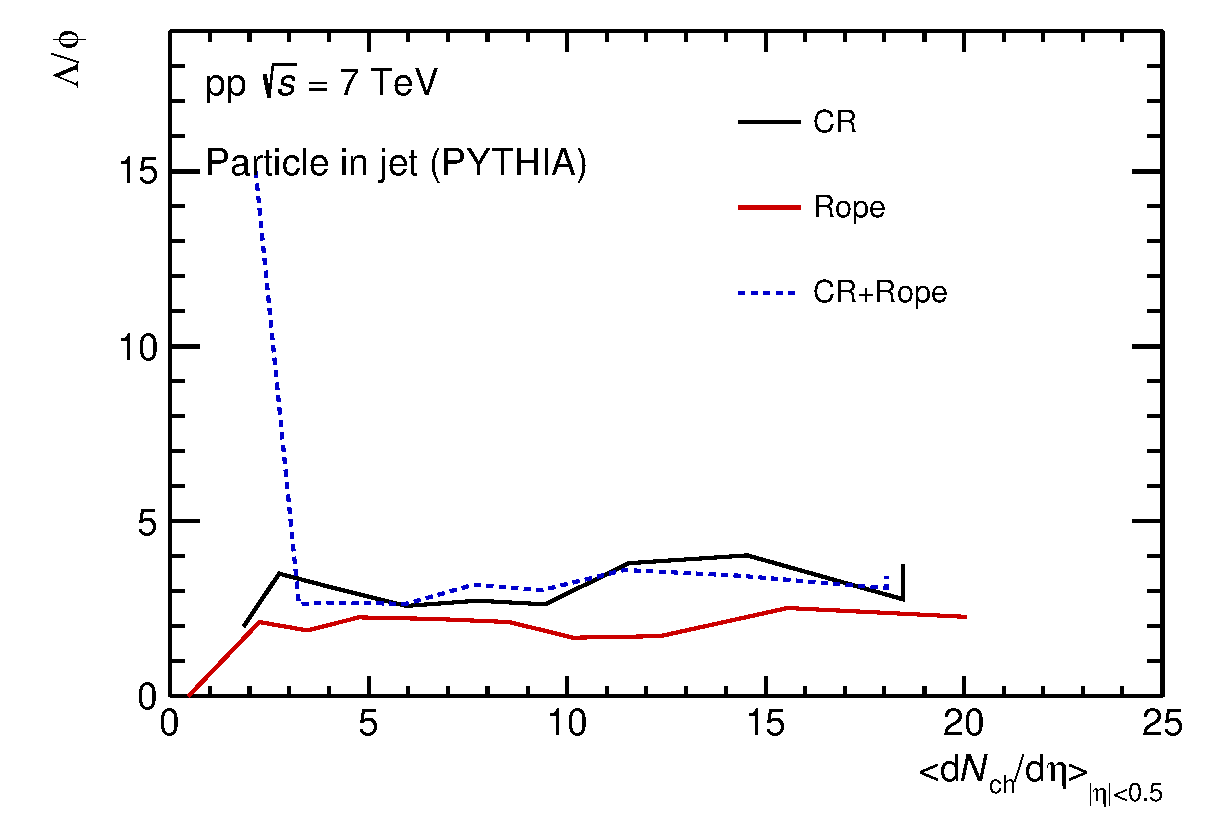
\includegraphics[width=.48\textwidth]{Inte_LambdaPhiRatio_JE}
		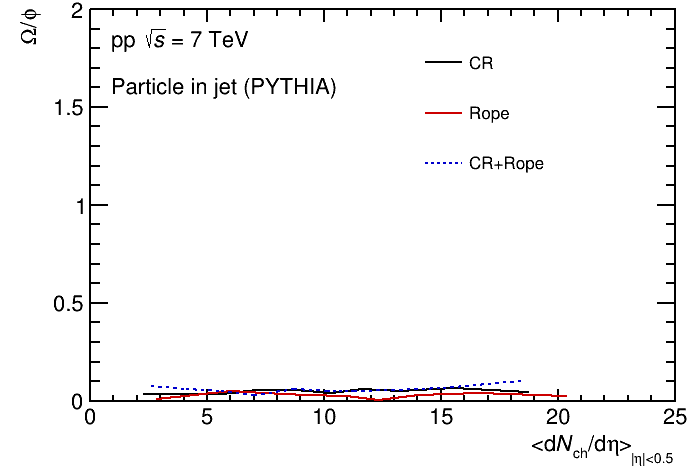
\includegraphics[width=.48\textwidth]{Inte_OmegaPhiRatio_JE}
		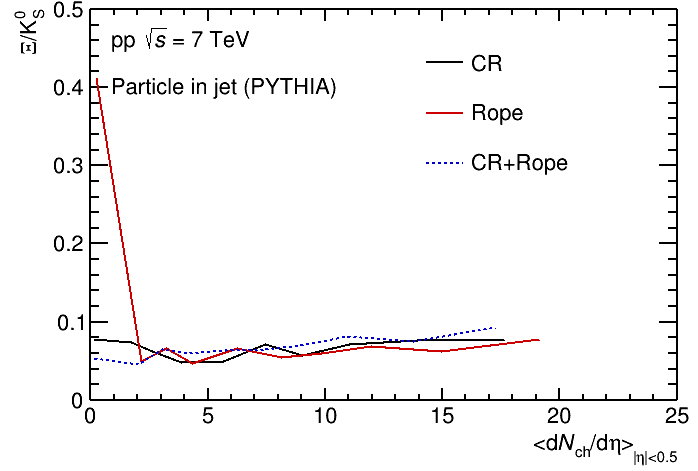
\includegraphics[width=.48\textwidth]{Inte_XiKshortRatio_JE}
		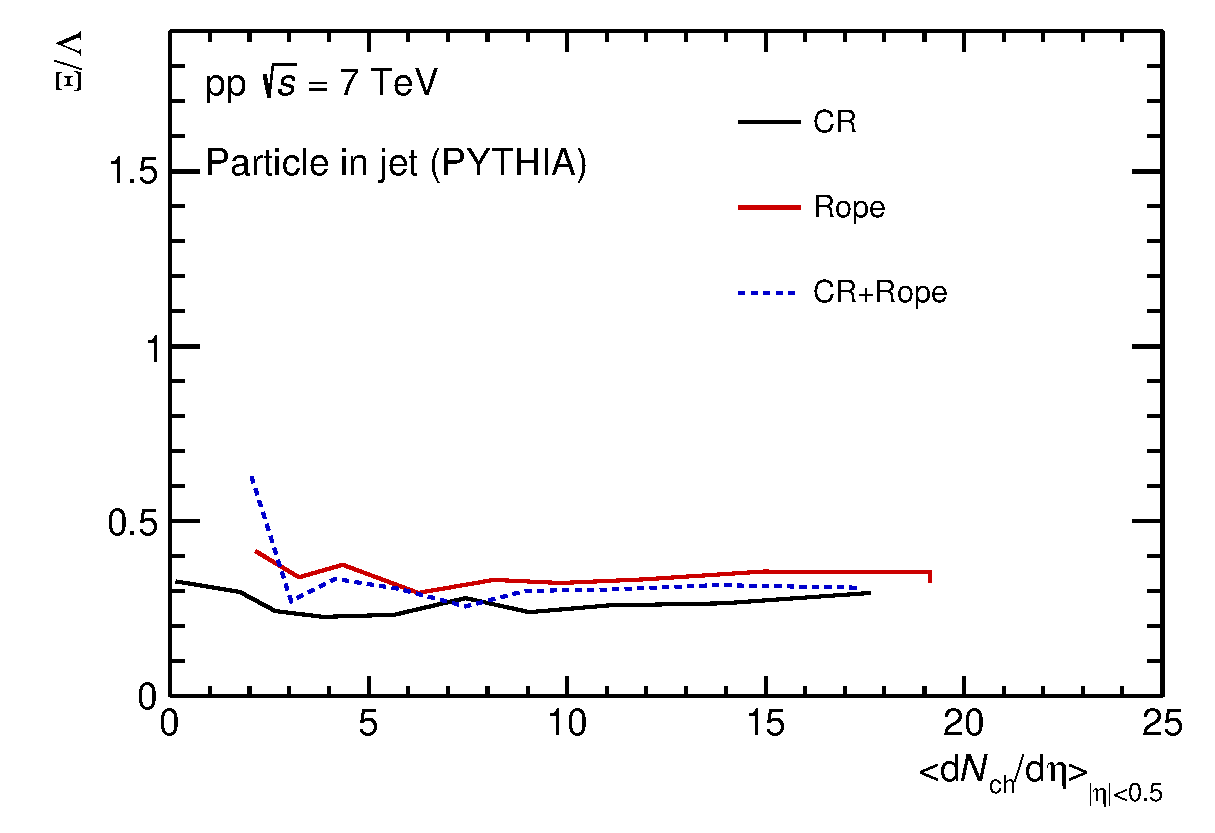
\includegraphics[width=.48\textwidth]{Inte_XiLambdaRatio_JE}
		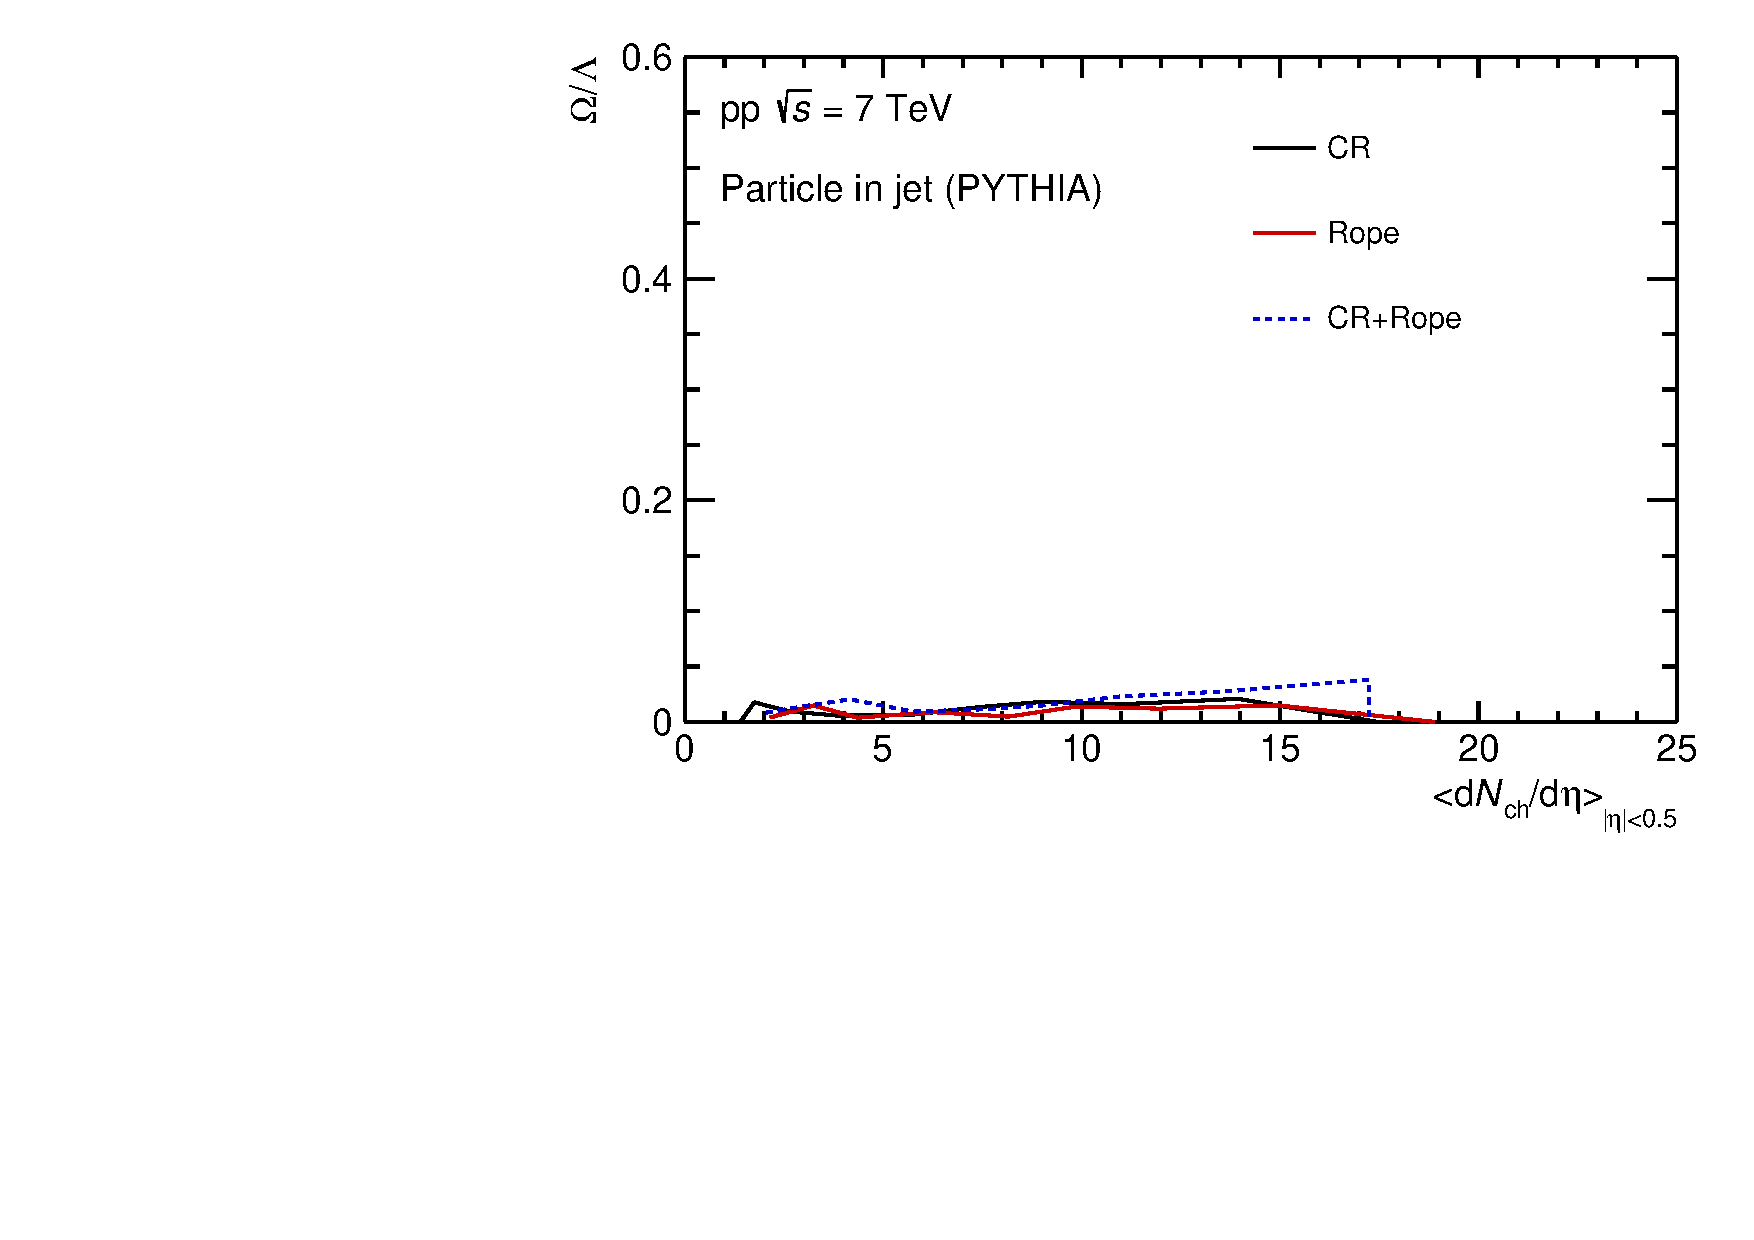
\includegraphics[width=.48\textwidth]{Inte_OmegaLambdaRatio_JE}
	\end{center}
	\caption{JC integrated yields ratios with $\avdndeta$.(Data taken from arXiv:1910.14397v1)}
	\label{fig:JCInteParRatio}
\end{figure}

%===================================================================
\begin{figure}[ht]
        \begin{center}
                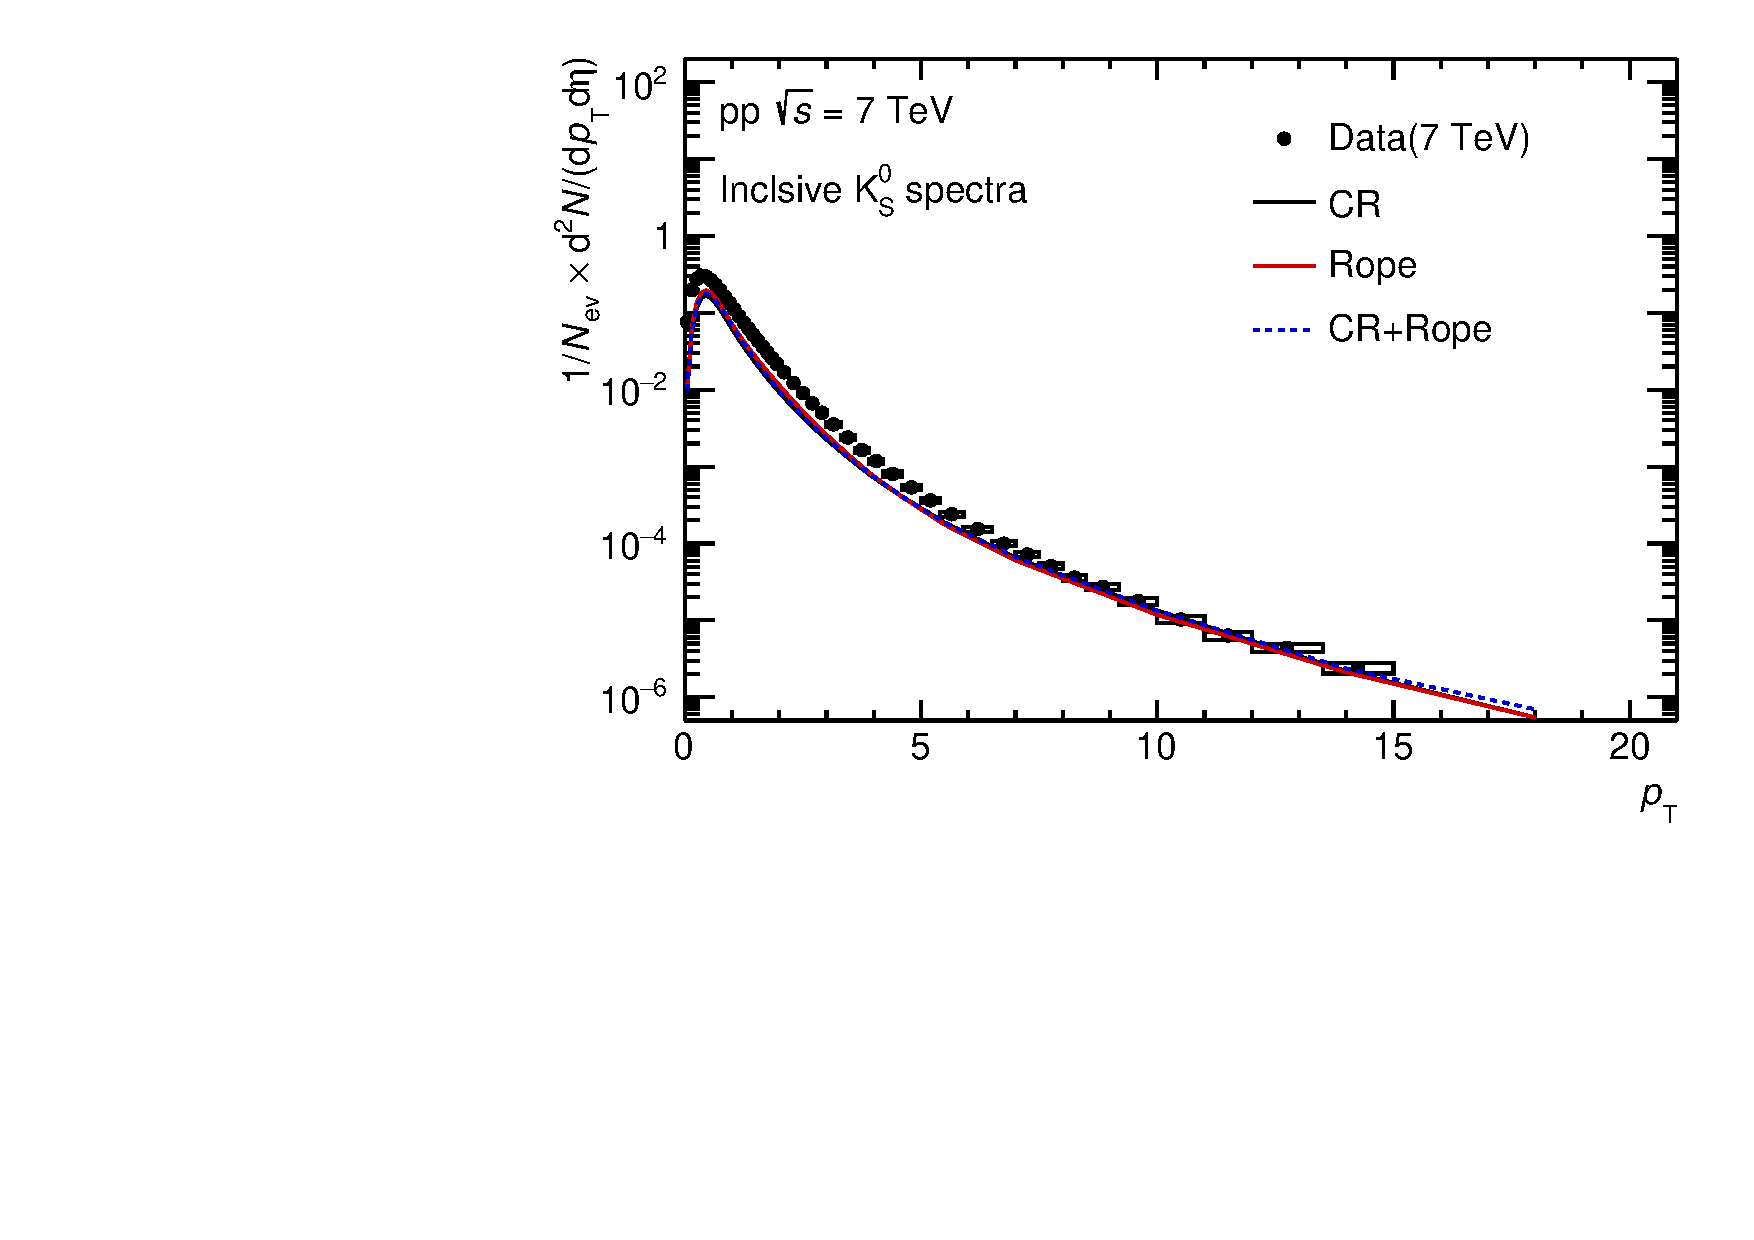
\includegraphics[width=.48\textwidth]{Incl_KshortSpect}
                \includegraphics[width=.48\textwidth]{Incl_LambdaSpect}
                \includegraphics[width=.48\textwidth]{Incl_XiSpect}
                \includegraphics[width=.48\textwidth]{Incl_OmegaSpect}
                \includegraphics[width=.48\textwidth]{Incl_KstarSpect}
                \includegraphics[width=.48\textwidth]{Incl_PhiSpect}
        \end{center}
	\caption{Inclusive particle $\pT$ spectra. The different acceptance with data(for PYTHIA $|\eta|<0.75$, data $|y|<0.5$)(Data taken from arXiv:2005.11120, arXiv:1204.0292v3 and arXiv:1910.14410)}
        \label{fig:InclParSpect}
\end{figure}


\begin{figure}[ht]
	\begin{center}
		\includegraphics[width=.48\textwidth]{JE_KshortSpect}
		\includegraphics[width=.48\textwidth]{JE_LambdaSpect}
		\includegraphics[width=.48\textwidth]{JE_XiSpect}
		\includegraphics[width=.48\textwidth]{JE_OmegaSpect}
		\includegraphics[width=.48\textwidth]{JE_KstarSpect}
		\includegraphics[width=.48\textwidth]{JE_PhiSpect}
	\end{center}
	\caption{Particle in jet $\pT$ spectra.}
	\label{fig:JEParSpect}
\end{figure}

%===================================================================
\begin{figure}[ht]
        \begin{center}
                \includegraphics[width=.42\textwidth]{LKRatio_Incl}
                \includegraphics[width=.42\textwidth]{XKRatio_Incl}
                \includegraphics[width=.42\textwidth]{OKRatio_Incl}
                \includegraphics[width=.42\textwidth]{PhiKRatio_Incl}
                \includegraphics[width=.42\textwidth]{KstarKRatio_Incl}
                \includegraphics[width=.42\textwidth]{XLRatio_Incl}
                \includegraphics[width=.42\textwidth]{OLRatio_Incl}
                \includegraphics[width=.42\textwidth]{OXRatio_Incl}
                \includegraphics[width=.42\textwidth]{XPhiRatio_Incl}
                \includegraphics[width=.42\textwidth]{OPhiRatio_Incl}
                %\includegraphics[width=.32\textwidth]{ProtonPionRatio_Incl}
        \end{center}
	\caption{Inclusive particle ratios with $\pT$ distribution. (Data taken from arXiv:2005.11120)}
        \label{fig:InclParRatio}
\end{figure}

\begin{figure}[ht]
        \begin{center}
                \includegraphics[width=.42\textwidth]{LKRatio_JE}
                \includegraphics[width=.42\textwidth]{XKRatio_JE}
                \includegraphics[width=.42\textwidth]{OKRatio_JE}
                \includegraphics[width=.42\textwidth]{PhiKRatio_JE}
                \includegraphics[width=.42\textwidth]{KstarKRatio_JE}
                \includegraphics[width=.42\textwidth]{XLRatio_JE}
                \includegraphics[width=.42\textwidth]{OLRatio_JE}
                \includegraphics[width=.42\textwidth]{OXRatio_JE}
                \includegraphics[width=.42\textwidth]{XPhiRatio_JE}
                \includegraphics[width=.42\textwidth]{OPhiRatio_JE}
                %\includegraphics[width=.32\textwidth]{ProtonPionRatio_Incl}
        \end{center}
	\caption{Particle ratios in jet with $\pT$ distribution. (Data taken from arXiv:2005.11120)}
        \label{fig:JEParRatio}
\end{figure}

%===================================================================
\begin{figure}[ht]
	\begin{center}
		\includegraphics[width=.48\textwidth]{LKRatio_Incl_Center}
		\includegraphics[width=.48\textwidth]{LKRatio_Incl_Peripheral}
		\includegraphics[width=.48\textwidth]{PhiKRatio_Incl_Center}
		\includegraphics[width=.48\textwidth]{PhiKRatio_Incl_Peripheral}
		\includegraphics[width=.48\textwidth]{KstarKRatio_Incl_Center}
		\includegraphics[width=.48\textwidth]{KstarKRatio_Incl_Peripheral}
	\end{center}
  \caption{Inclusive particle ratios  with $\pT$ distribution in center and peripheral centrality bins. (Data taken from arXiv:1807.11321v2 and arXiv:1910.14397v1)}
  \label{fig:InclParRatioCentPeri}
\end{figure}

%===================================================================

\begin{figure}[ht]
        \begin{center}
                \includegraphics[width=.42\textwidth]{LKRatio_Incl_Cent_cr_rope}
                \includegraphics[width=.42\textwidth]{XKRatio_Incl_Cent_cr_rope}
                \includegraphics[width=.42\textwidth]{OKRatio_Incl_Cent_cr_rope}
                \includegraphics[width=.42\textwidth]{KstarKRatio_Incl_Cent_cr_rope}
                \includegraphics[width=.42\textwidth]{PhiKRatio_Incl_Cent_cr_rope}
                \includegraphics[width=.42\textwidth]{XPhiRatio_Incl_Cent_cr_rope}
                \includegraphics[width=.42\textwidth]{OPhiRatio_Incl_Cent_cr_rope}
                \includegraphics[width=.42\textwidth]{XLRatio_Incl_Cent_cr_rope}
                \includegraphics[width=.42\textwidth]{OLRatio_Incl_Cent_cr_rope}
                \includegraphics[width=.42\textwidth]{OXRatio_Incl_Cent_cr_rope}
        \end{center}
	\caption{Particle ratios with $\pT$ distribution in different centrality bins (CR + Rope).}
        \label{fig:InclParRatioCentcrandrope}
\end{figure}
\begin{figure}[ht]
        \begin{center}
                \includegraphics[width=.42\textwidth]{LKRatio_Incl_Cent_cr}
                \includegraphics[width=.42\textwidth]{XKRatio_Incl_Cent_cr}
                \includegraphics[width=.42\textwidth]{OKRatio_Incl_Cent_cr}
                \includegraphics[width=.42\textwidth]{KstarKRatio_Incl_Cent_cr}
                \includegraphics[width=.42\textwidth]{PhiKRatio_Incl_Cent_cr}
                \includegraphics[width=.42\textwidth]{XPhiRatio_Incl_Cent_cr}
                \includegraphics[width=.42\textwidth]{OPhiRatio_Incl_Cent_cr}
                \includegraphics[width=.42\textwidth]{XLRatio_Incl_Cent_cr}
                \includegraphics[width=.42\textwidth]{OLRatio_Incl_Cent_cr}
                \includegraphics[width=.42\textwidth]{OXRatio_Incl_Cent_cr}
        \end{center}
	\caption{Particle ratios with $\pT$ distribution in different centrality bins (CR).}
        \label{fig:InclParRatioCentcr}
\end{figure}
\begin{figure}[ht]
        \begin{center}
                \includegraphics[width=.42\textwidth]{LKRatio_Incl_Cent_rope}
                \includegraphics[width=.42\textwidth]{XKRatio_Incl_Cent_rope}
                \includegraphics[width=.42\textwidth]{OKRatio_Incl_Cent_rope}
                \includegraphics[width=.42\textwidth]{KstarKRatio_Incl_Cent_rope}
                \includegraphics[width=.42\textwidth]{PhiKRatio_Incl_Cent_rope}
                \includegraphics[width=.42\textwidth]{XPhiRatio_Incl_Cent_rope}
                \includegraphics[width=.42\textwidth]{OPhiRatio_Incl_Cent_rope}
                \includegraphics[width=.42\textwidth]{XLRatio_Incl_Cent_rope}
                \includegraphics[width=.42\textwidth]{OLRatio_Incl_Cent_rope}
                \includegraphics[width=.42\textwidth]{OXRatio_Incl_Cent_rope}
        \end{center}
	\caption{Particle ratios with $\pT$ distribution in different centrality bins (Rope).}
        \label{fig:InclParRatioCentrope}
\end{figure}
%===================================================================


\begin{figure}[ht]
        \begin{center}
                \includegraphics[width=.42\textwidth]{LKRatio_JE_Cent_cr_rope}
                \includegraphics[width=.42\textwidth]{XKRatio_JE_Cent_cr_rope}
                \includegraphics[width=.42\textwidth]{OKRatio_JE_Cent_cr_rope}
                \includegraphics[width=.42\textwidth]{KstarKRatio_JE_Cent_cr_rope}
                \includegraphics[width=.42\textwidth]{PhiKRatio_JE_Cent_cr_rope}
                \includegraphics[width=.42\textwidth]{XPhiRatio_JE_Cent_cr_rope}
                \includegraphics[width=.42\textwidth]{OPhiRatio_JE_Cent_cr_rope}
                \includegraphics[width=.42\textwidth]{XLRatio_JE_Cent_cr_rope}
                \includegraphics[width=.42\textwidth]{OLRatio_JE_Cent_cr_rope}
                \includegraphics[width=.42\textwidth]{OXRatio_JE_Cent_cr_rope}
        \end{center}
	\caption{Particle ratios in jet with $\pT$ distribution in different centrality bins (CR+Rope).}
        \label{fig:JEParRatioCentcrandrope}
\end{figure}

\begin{figure}[ht]
        \begin{center}
                \includegraphics[width=.42\textwidth]{LKRatio_JE_Cent_cr}
                \includegraphics[width=.42\textwidth]{XKRatio_JE_Cent_cr}
                \includegraphics[width=.42\textwidth]{OKRatio_JE_Cent_cr}
                \includegraphics[width=.42\textwidth]{KstarKRatio_JE_Cent_cr}
                \includegraphics[width=.42\textwidth]{PhiKRatio_JE_Cent_cr}
                \includegraphics[width=.42\textwidth]{XPhiRatio_JE_Cent_cr}
                \includegraphics[width=.42\textwidth]{OPhiRatio_JE_Cent_cr}
                \includegraphics[width=.42\textwidth]{XLRatio_JE_Cent_cr}
                \includegraphics[width=.42\textwidth]{OLRatio_JE_Cent_cr}
                \includegraphics[width=.42\textwidth]{OXRatio_JE_Cent_cr}
        \end{center}
	\caption{Particle ratios in jet with $\pT$ distribution in different centrality bins (CR).}
        \label{fig:JEParRatioCentcr}
\end{figure}
\begin{figure}[ht]
        \begin{center}
                \includegraphics[width=.42\textwidth]{LKRatio_JE_Cent_rope}
                \includegraphics[width=.42\textwidth]{XKRatio_JE_Cent_rope}
                \includegraphics[width=.42\textwidth]{OKRatio_JE_Cent_rope}
                \includegraphics[width=.42\textwidth]{KstarKRatio_JE_Cent_rope}
                \includegraphics[width=.42\textwidth]{PhiKRatio_JE_Cent_rope}
                \includegraphics[width=.42\textwidth]{XPhiRatio_JE_Cent_rope}
                \includegraphics[width=.42\textwidth]{OPhiRatio_JE_Cent_rope}
                \includegraphics[width=.42\textwidth]{XLRatio_JE_Cent_rope}
                \includegraphics[width=.42\textwidth]{OLRatio_JE_Cent_rope}
                \includegraphics[width=.42\textwidth]{OXRatio_JE_Cent_rope}
        \end{center}
	\caption{Particle ratios in jet with $\pT$ distribution in different centrality bins (Rope).}
        \label{fig:JEParRatioCentrope}
\end{figure}

\begin{figure}[ht]
	\begin{center}
                \includegraphics[width=.42\textwidth]{LK_toJetRange}
                \includegraphics[width=.42\textwidth]{XK_toJetRange}
                \includegraphics[width=.42\textwidth]{OK_toJetRange}
                \includegraphics[width=.42\textwidth]{KstarK_toJetRange}
                \includegraphics[width=.42\textwidth]{PhiK_toJetRange}
                \includegraphics[width=.42\textwidth]{XPhi_toJetRange}
                \includegraphics[width=.42\textwidth]{OPhi_toJetRange}
                \includegraphics[width=.42\textwidth]{XL_toJetRange}
                \includegraphics[width=.42\textwidth]{OL_toJetRange}
                \includegraphics[width=.42\textwidth]{OX_toJetRange}
	\end{center}
	\caption{Particle ratios to jet axis range ($R$(P, jet)) distribution. (The multi-strange hadrons ($\Xi$, $\Omega$) have strong enhance at small $R$(P, jet))}
	\label{fig:ParRatiotoJet}
\end{figure}

\begin{figure}[ht]
	\begin{center}
		\includegraphics[width=.42\textwidth]{LK_toJetRange_cent_CR}
		\includegraphics[width=.42\textwidth]{XK_toJetRange_cent_CR}
		\includegraphics[width=.42\textwidth]{OK_toJetRange_cent_CR}
		\includegraphics[width=.42\textwidth]{KstarK_toJetRange_cent_CR}
		\includegraphics[width=.42\textwidth]{PhiK_toJetRange_cent_CR}
		\includegraphics[width=.42\textwidth]{XPhi_toJetRange_cent_CR}
		\includegraphics[width=.42\textwidth]{OPhi_toJetRange_cent_CR}
		\includegraphics[width=.42\textwidth]{XL_toJetRange_cent_CR}
		\includegraphics[width=.42\textwidth]{OL_toJetRange_cent_CR}
		\includegraphics[width=.42\textwidth]{OX_toJetRange_cent_CR}
	\end{center}
	\caption{Particle ratios to jet axis range ($R$(P, jet)) distribution. (The multi-strange hadrons ($\Xi$, $\Omega$) have strong enhance at small $R$(P, jet))}
	\label{fig:ParRatiotoJetCR}
\end{figure}

\begin{figure}[ht]
\begin{center}
	\includegraphics[width=.42\textwidth]{LK_toJetRange_cent_CRandRope}
	\includegraphics[width=.42\textwidth]{XK_toJetRange_cent_CRandRope}
	\includegraphics[width=.42\textwidth]{OK_toJetRange_cent_CRandRope}
	\includegraphics[width=.42\textwidth]{KstarK_toJetRange_cent_CRandRope}
	\includegraphics[width=.42\textwidth]{PhiK_toJetRange_cent_CRandRope}
	\includegraphics[width=.42\textwidth]{XPhi_toJetRange_cent_CRandRope}
	\includegraphics[width=.42\textwidth]{OPhi_toJetRange_cent_CRandRope}
	\includegraphics[width=.42\textwidth]{XL_toJetRange_cent_CRandRope}
	\includegraphics[width=.42\textwidth]{OL_toJetRange_cent_CRandRope}
	\includegraphics[width=.42\textwidth]{OX_toJetRange_cent_CRandRope}
\end{center}
\caption{Particle ratios to jet axis range ($R$(P, jet)) distribution. (The multi-strange hadrons ($\Xi$, $\Omega$) have strong enhance at small $R$(P, jet))}
\label{fig:ParRatiotoJetCRandRope}
\end{figure}
\begin{figure}[ht]
\begin{center}
	\includegraphics[width=.42\textwidth]{LK_toJetRange_cent_Rope}
	\includegraphics[width=.42\textwidth]{XK_toJetRange_cent_Rope}
	\includegraphics[width=.42\textwidth]{OK_toJetRange_cent_Rope}
	\includegraphics[width=.42\textwidth]{KstarK_toJetRange_cent_Rope}
	\includegraphics[width=.42\textwidth]{PhiK_toJetRange_cent_Rope}
	\includegraphics[width=.42\textwidth]{XPhi_toJetRange_cent_Rope}
	\includegraphics[width=.42\textwidth]{OPhi_toJetRange_cent_Rope}
	\includegraphics[width=.42\textwidth]{XL_toJetRange_cent_Rope}
	\includegraphics[width=.42\textwidth]{OL_toJetRange_cent_Rope}
	\includegraphics[width=.42\textwidth]{OX_toJetRange_cent_Rope}
\end{center}
\caption{Particle ratios to jet axis range ($R$(P, jet)) distribution. (The multi-strange hadrons ($\Xi$, $\Omega$) have strong enhance at small $R$(P, jet))}
\label{fig:ParRatiotoJetRope}
\end{figure}